\documentclass[11pt]{article}

\usepackage{maiacustom}

\begin{document}

\psettitle{Banco de questões de astronomia}

Estas questões foram produzidas/selecionadas cuidadosamente com o objetivo de preparar os estudantes para o processo seletivo de astronomia no Brasil. Algumas questões não são de autoria própria e estão devidamente sinalizadas por () antes do enunciado. O template do banco de questões é o mesmo do Professor \text{Kevin Zhou}. Seu trabalho é valioso, e diversas ideias desta lista podem ser encontradas em seus Handouts.

% \begin{psidea}{Título da Ideia}{}
% Ideia
% \end{psidea}

% \begin{psexample}{Título do Exemplo}{}
% Exemplo
% \end{psexample}

% \begin{pssolution*}{}{}
% Solução
% \end{pssolution*}

% \begin{psremark*}{Título da Observação}{}
% Observação
% \end{psremark*} 

\section{Mecânica Celeste}
\pts{5}    
\begin{pproblem}
    Iaum e Sevla, dois físicos renomados, pretendem lançar uma sonda espacial para explorar os limites da física newtoniana e as correções relativísticas necessárias nas proximidades de um buraco negro. Eles precisam da sua ajuda para estudar o \textit{Potencial Efetivo} de tal corpo.
    \begin{enumerate}[label=\textbf{\alph*)}]
        \item A energia de um corpo de massa \(m\) orbitando um corpo massivo de massa \(M\) pode ser escrita como:
             \[
             \frac{m\dot r ^2}{2} + V_{eff}(r)
             \]
             Onde \(\dot r\) é a velocidade radial do corpo. Encontre \(V_{eff}(r)\) em função de \(G\), \(M\), \(L\), \(m\) e \(r\).

        \item Segundo a física newtoniana, qual é o menor raio no qual é possível um corpo possuir uma órbita circular em torno de um buraco negro?
    
        \item Qual é a frequência de pequenas oscilações radiais, \(\omega_r\), em torno desse raio?

        O potencial gravitacional próximo a esses corpos precisa sofrer uma correção relativística e tem a forma:
        \[
        V(r) = -\frac{GMm}{r} - \frac{GML^2}{mc^2r^3}
        \]

        \item Explique por que essa correção permite que uma partícula caia no centro de um buraco negro, \(r=0\), e por que isso é impossível na física newtoniana.
        
        \item Qual é o menor valor de \(L\) para que uma partícula possa orbitar o buraco negro em uma órbita circular? Qual é o valor do raio nessa condição?
        
        \item Assumindo \( \lim_{L \to \infty}\), encontre a menor distância que uma partícula em órbita aberta pode se aproximar de um buraco negro.  
    \end{enumerate}
    \begin{pssolution*}{}{}
        \begin{alternativas}
            \item Da forma clássica, temos:
            \[E = \frac{mv^2}{2}-\frac{GMm}{r}\]
            Note que podemos escrever \(v^2 = v_\theta^2+ v_r^2\), onde \(v_\theta\) e \(v_r\) são, respectivamente, as velocidades tangenciais e radiais do corpo. Como \(v_r = \dot{r}\), precisamos encontrar uma expressão que relacione \(v_\theta\) com outra grandeza. A melhor maneira de fazer essa relação é utilizando o momento angular, pois:
            \[L = mrv_\theta \rightarrow v_\theta = \frac{L}{mr}\]
            Substituindo na expressão da energia, temos:
            \[E = \frac{m\dot{r}^2}{2}+\frac{L^2}{2mr^2} - \frac{GMm}{r}\]
            Como queremos uma resposta na forma \(E = m\dot{r}^2/2 + V_{eff}(r)\), por analogia, temos:
            \[\boxed{V_{eff}(r) = -\frac{GMm}{r}+\frac{L^2}{2mr^2}}\]

            \item A maior velocidade limite de um corpo é \(c\), desconsiderando efeitos relativísticos:
            \[\frac{mc^2}{2}-\frac{GMm}{R} = -\frac{GMm}{2R}\]
            Isolando \(R\):
            \[\boxed{R = \frac{GM}{c^2}}\]

            \item Para pequenas oscilações, temos a aproximação:
            \[\omega_r \approx \sqrt{\frac{V_{eff}''(R)}{m}}\]
            Calculando:
            \[V_{eff}'(R) = \frac{GMm}{r^2}-\frac{L^2}{mr^3}\]
            \[V_{eff}''(R) = -\frac{2GMm}{r^3}+\frac{3L^2}{mr^4}\]
            Utilizando que \(L = mvr\) (órbitas circulares) e que \(v\equiv c\), chegamos a:
            \[V_{eff}''(R) = \frac{mc^6}{G^2M^2}\]
            Com isso, podemos concluir que:
            \[\omega_r = \frac{c^3}{GM}\]

            \item Quando tomamos o limite de \(\lim_{r\rightarrow 0}V_{eff}(r)\), na física newtoniana, o termo que domina é \(L^2/2mr^2\), ou seja, seria necessária uma energia \(+\infty\) para chegar ao centro do buraco negro. No entanto, após a correção relativística, o termo que domina é \(-GML^2/mc^2r^3\), ou seja, seria necessária uma energia de \(-\infty\) para chegar ao centro do buraco negro. Por isso, não é possível chegar ao centro de um buraco negro na física newtoniana.
            
            \item Em uma órbita circular, \(r\) é constante, o que implica que a força na direção radial é nula, ou seja:
            \[V_{eff}'(r) = 0\]
            Calculando:
            \[V_{eff}'(r) = \frac{GMm}{r^2}-\frac{L^2}{mr^3}+\frac{3GML^2}{mc^2r^4}=0\]
            Simplificando, temos:
            \[r^2-\frac{L^2}{GMm^2}r+\frac{3L^2}{m^2c^2}=0\]
            Note que a solução dessa equação precisa ser real, uma vez que \(r\) não pode ser imaginário, o que nos impõe a condição:
            \[\frac{L^4}{G^2M^2m^4} - \frac{12L^2}{m^2c^2} \geq 0\]
            Na condição de igualdade, o valor de \(L\) que satisfaz essa equação é:
            \[\boxed{L = \frac{\sqrt{12}GMm}{c}}\]
            O valor de \(r\) nesse caso é:
            \[r = \frac{L^2}{2GMm^2} = \boxed{r_{min} = \frac{6GM}{c^2}}\] 
            
            \item A expressão completa para \(r\) é:
            \[r = \frac{\frac{L^2}{GMm^2}\pm\sqrt{\left(\frac{L^2}{GMm^2}\right)^2-\frac{12L^2}{m^2c^2}}}{2} = \frac{L^2-\sqrt{L^4-12(GMmL/c)^2}}{2GMm^2}\] 
            No limite de \(L\rightarrow \infty\), temos:
            \[r_{min} = \lim_{L \rightarrow \infty}\frac{L^2-\sqrt{L^4-12(GMmL/c)^2}}{2GMm^2} = \frac{6(GMm/c)^2}{2(GMm^2)} = \boxed{\frac{3GM}{c^2}} \] 
        \end{alternativas}
    \end{pssolution*}
\end{pproblem}

\pts{3}
\begin{pproblem} Um ponto importante no estudo de órbitas é o que acontece quando o potencial segue algo incomum. O objetivo desta questão é estudar esse fenômeno. Considere o momento angular \(L\) e a massa do corpo \(m\).
    \begin{alternativas}
        \item Para uma órbita geral, que possui um potencial \(V(r)\) na forma \(\psi r^k\), encontre o valor \(r_0\) de uma órbita circular para esse potencial.
        
        \item Encontre a frequência de pequenas oscilações, \(\omega_r\), em torno desse raio. 
        
        \item Seja \(\omega_\theta\) a frequência angular da órbita, encontre o valor da razão \(\frac{\omega_r}{\omega_\theta}\). Uma órbita só pode ser fechada se essa razão for um número inteiro. Por quê? Encontre valores de \(k\) para que a órbita seja fechada.
         
    \end{alternativas} 

    \begin{pssolution*}{}{}
        \begin{alternativas}
            \item Como em uma órbita circular \(V_{eff}'(r) = 0\), temos:
            \[V_{eff}'(r) = -\frac{L^2}{mr^3}+k\psi r^{k-1} = 0\]
            \[k\psi r^{k-1} = \frac{L^2}{mr^3} \rightarrow \boxed{r_0 = \left(\frac{L^2}{k\psi m}\right)^{\frac{1}{k+2}}}\]
        
            \item Utilizando que \(\omega_r^2=V_{eff}''(r_0)/m\):
            \[V_{eff}''(r) = \frac{3L^2}{mr^4}+k(k-1)\psi r^{k-2}\]
            \[V_{eff}''(r) = r^{-4}\left(\frac{3L^2}{m}+k(k-1)\psi r^{k+2}\right)\]
            \[V_{eff}''(r) = r^{-4}\left(\frac{3L^2}{m}+k(k-1)\psi \frac{L^2}{k\psi m}\right)\]
            \[V_{eff}''(r) = \frac{L^2}{r_0^4m}(k+2)\]
            Assim, temos:
            \[\boxed{\omega_r = \frac{L}{r_0^2m}\sqrt{k+2}}\]

            \item Pela definição de \(L\), temos:
            \[L = mr_0^2\omega_\theta \rightarrow \omega_\theta = \frac{L}{mr_0^2}\]
            Portanto:
            \[\frac{\omega_r}{\omega_\theta} = \sqrt{k+2}\]
            Note que, para a órbita ser uma figura fechada, essa razão deve ser um número inteiro, logo, \(k+2\) deve ser um quadrado perfeito. Qualquer valor \(k = n^2-2 \ \forall \ n \in \mathbb{N}\) satisfaz essa equação.
        \end{alternativas}
    \end{pssolution*}
\end{pproblem}

\pts{4} %semana 114
\begin{pproblem}
    O Hodógrafo é uma das maneiras menos conhecidas de resolver questões de mecânica celeste. Ao usar esse mecanismo, é possível resolver questões complexas (envolvendo encontrar parâmetros orbitais, parâmetros de velocidade e como minimizar a excentricidade de uma órbita, por exemplo). Apesar de o Hodógrafo possuir diversas utilidades, o objetivo deste exercício é provar o Teorema do Hodógrafo, que diz que, em órbitas fechadas, a velocidade forma um círculo no espaço vetorial. Vamos provar esse teorema de duas maneiras.
    \begin{align*}
    \textbf{Método 1)}
    \end{align*}
    \begin{enumerate}[label=\textbf{\Roman*.}]
        \item Partindo da Segunda Lei de Newton e da conservação do momento angular, encontre uma expressão para \(d\mathbf{v}/d\theta\). Deixe sua resposta em função do momento angular por unidade de massa, \(h\), e \(\mu\) = \(GM\). 
        \item Onde o centro desse círculo está localizado? Considerando o corpo central na origem do sistema, determine uma expressão para a distância entre o corpo central e o centro do Hodógrafo. 
    \end{enumerate}
    
    \begin{align*}
        \textbf{Método 2)}
    \end{align*}
    O método 2 utiliza noções de cálculo mais avançadas e parte da conservação do \textit{vetor de Laplace-Runge-Lenz}, \(\mathbf{A}\).
    \begin{enumerate}[label=\textbf{\Roman*.}]
        \item O vetor \(\mathbf{A}\) é dado pela expressão:
        \[
        \mathbf{A} = \mathbf{p}\times \mathbf{L} - GMm^2\mathbf{\hat{r}}
        \]
        O primeiro passo para a demonstração é provar que \(\mathbf{A}\) é constante. Para isso, derive o mesmo em relação ao tempo e tire suas próprias conclusões.
        \item Como o vetor \(\mathbf{L}\) é constante, \(\mathbf{A}\times\mathbf{L}\) também é uma constante. Utilizando a identidade vetorial \(\mathbf{A}\times(\mathbf{B}\times\mathbf{C}) = \mathbf{B}(\mathbf{A}\cdot\mathbf{C}) - \mathbf{C}(\mathbf{A}\cdot\mathbf{B}) \), prove que \(\mathbf{v}\) forma um círculo no espaço vetorial.    
    \end{enumerate}
    \begin{pssolution*}{}{}
        \textbf{Método 1)}

        \begin{enumerate}[label=\textbf{\Roman*.}]
            \item A Segunda Lei de Newton nos diz que:
            \[-\frac{GMm}{r^2}\mathbf{\hat{r}} =  m\frac{d\mathbf{v}}{dt}\]
            Pela definição de momento angular:
            \[L = mr^2\frac{d\theta}{dt} \rightarrow \ \  \therefore dt = \frac{mr^2}{L}d\theta\]
            Substituindo \(dt\) na fórmula da Segunda Lei de Newton:
            \[-\frac{GMm}{r^2}\mathbf{\hat{r}} = m\left(\frac{L}{mr^2}\right)\frac{d\mathbf{v}}{d\theta}\]

            Isolando \(dv/d\theta\), temos:

            \[\boxed{\frac{d\mathbf{v}}{d\theta} = -\frac{GMm}{L}\mathbf{\hat{r}} \equiv -\frac{\mu}{h}\mathbf{\hat{r}}}\]

            Note que essa expressão é um círculo no espaço vetorial e possui raio \(R = \mu/h\), uma vez que \(d\mathbf{v}/d\theta\) é constante e aponta na direção radial.

            \item Como vimos no item anterior, o hodógrafo forma um círculo de raio \(R = \mu/h\). Tome como apoio a seguinte imagem:
            \begin{figure}[H]
                \centering
                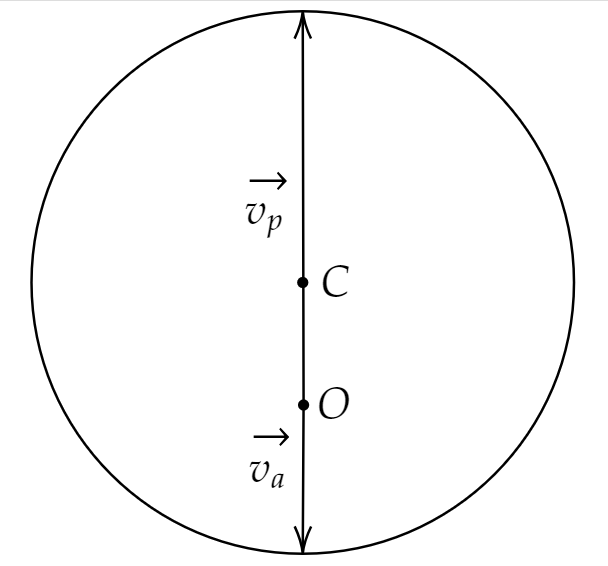
\includegraphics[width=0.4\linewidth]{imagens/hodografo1.png}
                \caption{Esquema do Hodógrafo}
            \end{figure}
            O ponto \(O\) representa a origem do sistema (local do corpo central). Note que a menor distância entre \(O\) e o Hodógrafo deve corresponder à menor velocidade (apoastro) e a maior distância deve corresponder à maior velocidade (periastro). Note também que \(v_a + \overline{OC} = v_p - \overline{OC}\). Equacionando, temos:
            \[v_a + v_p = 2R \equiv \frac{2\mu}{h}\]
            \[v_p - v_a = 2\overline{OC}\]

            Podemos escrever \(v_p\) e \(v_a\) em função do momento angular:
            \[L = ma(1-e)v_p \rightarrow v_p = \frac{h}{a(1-e)}\]
            \[L = ma(1+e)v_a \rightarrow v_a = \frac{h}{a(1+e)}\]
            
            Substituindo na primeira equação:
            \[\frac{h}{a}\left(\frac{1}{1+e}+\frac{1}{1-e}\right) = \frac{2\mu}{h}\]
            
            Aqui, podemos isolar \(a\):
            \[\frac{h}{a}\left(\frac{2}{(1-e)^2}\right) = \frac{2\mu}{h}\]

            \[a = \frac{h^2}{\mu}\frac{1}{(1-e)^2}\]

            Com isso em mente, podemos ir para a segunda expressão:
            \[\frac{h}{a}\left(\frac{1}{1-e}-\frac{1}{1+e}\right) = 2\overline{OC}\]
            \[h\left(\frac{\mu(1-e)^2}{h^2}\right)\left(\frac{2e}{(1-e)^2}\right) = 2\overline{OC}\]
            
            Finalmente, resolvendo para \(\overline{OC}\), temos:
            \[\boxed{\overline{OC} = \frac{\mu}{h}e}\]

            Para uma elipse (\(e<1\)), a origem fica dentro da circunferência; para uma parábola (\(e=1\)), a origem fica no limite da circunferência; e para uma hipérbole (\(e>1\)), a origem fica fora da circunferência.
        \end{enumerate}

    
        \textbf{Método 2}
        \begin{enumerate}[label=\textbf{\Roman*.}]
            \item Derivando \(\mathbf{A}\) em relação ao tempo, temos:
            \[\frac{d\mathbf{A}}{dt} = \frac{d}{dt}(\mathbf{p}\times\mathbf{L}) - GMm^2\frac{d}{dt}\mathbf{\hat{r}}\] 
            Quando derivamos um \textit{versor} em relação ao tempo, temos:
            \[\frac{d\mathbf{\hat{r}}}{dt} = \mathbf{\omega}\times\mathbf{\hat{r}}\]
            Onde \(\mathbf{\omega}\) é a velocidade com que o versor translada. Assim:
            \[\frac{d\mathbf{A}}{dt} = \left(\frac{d\mathbf{p}}{dt}\right)\times \mathbf{L} + \mathbf{p}\times\left(\frac{d\mathbf{L}}{dt}\right) - GMm^2(\mathbf{\omega}\times \mathbf{\hat{r}})\]
            Agora, temos algumas considerações. Primeiramente, note que \(d\mathbf{L}/dt=0\), uma vez que só há forças centrais na órbita. Em segundo lugar, \(d\mathbf{p}/dt = \mathbf{F}\). Além disso, temos que \(\mathbf{L} = mr^2\mathbf{\omega}\). Voltando para a equação:

            \[\frac{d\mathbf{A}}{dt} = -\frac{GMm}{r^2}\mathbf{\hat{r}}\times(mr^2\mathbf{\omega}) - GMm^2(\mathbf{\omega} \times \mathbf{\hat{r}})\]
            \[\frac{d\mathbf{A}}{dt} = -GMm^2(\mathbf{\hat{r}}\times\mathbf{\omega})- GMm^2(\mathbf{\omega} \times \mathbf{\hat{r}})\]

            Para quaisquer dois vetores, \(\mathbf{i}\) e \(\mathbf{j}\), vale que:
            \[i\times j = -j\times i\]

            Utilizando tal propriedade, podemos concluir que:

            \[\boxed{\frac{d\mathbf{A}}{dt} = 0}\]

            Logo, \(\mathbf{A}\) é constante!

            \item Escrevendo a expressão e utilizando o \textit{BAC-CAB}, temos:
            
            \[\mathbf{A}\times\mathbf{L} = (\mathbf{p}\times\mathbf{L})\times\mathbf{L} - GMm^2\mathbf{\hat{r}}\times\mathbf{L}\]

            \[(\mathbf{A} +GMm^2\mathbf{\hat{r}})\times\mathbf{L} = - \mathbf{L}\times(\mathbf{p}\times\mathbf{L}) = \mathbf{p}(-\mathbf{L}\cdot\mathbf{L})-\mathbf{L}(-\mathbf{L}\cdot\mathbf{p})\]

            Como \(\mathbf{L}\) e \(\mathbf{p}\) são sempre perpendiculares, \(\mathbf{L}\cdot\mathbf{p}=0\), assim:

            \[(\mathbf{A}+GMm^2\mathbf{\hat{r}})\times\mathbf{L} = -mL^2\mathbf{v}\]

            Como tanto \(\mathbf{A}\) quanto \(\mathbf{\hat{r}}\) são perpendiculares a \(\mathbf{L}\) e constantes, \(\mathbf{A}+GMm^2\mathbf{\hat{r}}\) traçam um círculo. O produto vetorial com \(\mathbf{L}\) apenas gira o círculo em \(90^\circ\) e multiplica seu raio por \(\mathbf{L}\). Portanto, \(\mathbf{v}\) traça um círculo no espaço vetorial.
            
        \end{enumerate}
    \end{pssolution*}
\end{pproblem}

\pts{2} %problemas da semana 114
\begin{pproblem} Um dos fenômenos mais fascinantes do sistema solar são as estrelas de nêutrons. Esses são corpos muito pequenos, super densos e que giram muito rápido. Nesta questão, vamos fazer um modelo teórico para essas estrelas.
    \begin{enumerate}[label=\textbf{\alph*)}]
        \item O Pulsar da Vela, uma estrela de nêutrons localizada na constelação da Vela, possui uma frequência de \(11 \text{Hz}\), ou seja, ela gira em torno de si mesma \(11\) vezes por segundo, raio equatorial \(R_e = 9,6\text{ km}\) e massa \(M = 1,88M_\odot\). Sabendo disso, calcule a razão entre seu raio equatorial e seu raio polar.
        \item Qual é o menor período de rotação que o Pulsar da Vela pode ter para que ele não se despedace?
        \item Atualmente, a taxa de variação do período do Pulsar da Vela é \(\frac{\Delta P}{\Delta t} = 1,25 \cdot 10^{-13}\text{s/s}\). Isso faz com que o Pulsar libere uma quantidade absurda de energia. A temperatura superficial do Pulsar é de \(T \sim 10^6\text{ K}\). Calcule a ordem de grandeza da razão entre a potência emitida pelo aumento do período e a potência emitida pela Lei de Stefan-Boltzmann.
    \end{enumerate}
    \begin{pssolution*}{}{}
        \begin{alternativas}
            \item Uma estrela sempre está em equilíbrio hidrostático, logo, equacionando para um ponto no equador e para um dos polos,
            \[-\frac{GM}{r_e}-\frac{1}{2}\omega^2r_e^2 = -\frac{GM}{r_p}\]

            Utilizando que \(\omega = 2\pi f\),

            \[\frac{GM}{r_p} = \frac{GM}{r_e}+2\pi^2f^2r_e^2\]

            \[\boxed{\frac{r_e}{r_p} = 1+\frac{2\pi^2f^2r_e^3}{GM} \approx 1 + 8,4\cdot10^{-6}}\]

            Ou seja, uma estrela de nêutrons, mesmo girando absurdamente rápido, ainda é praticamente uma esfera perfeita!

            \item Na situação limite para se manter íntegro, temos:
            \[\frac{GM}{r_e^2} = \omega^2r_e\]
            \[\omega^2 = \frac{GM}{r_e^3} \rightarrow \boxed{T_{min} = \frac{2\pi r_e^3}{GM} = 2,2\cdot10^{-8}\text{ s}}\]

            \item A energia devido à rotação tem a forma:
            \[E = \frac{1}{2}I\omega^2\]
            Onde \(I\) é o momento de inércia da estrela (\(I = \frac{2}{5}Mr^2\)). Portanto, a potência dissipada é:
            \[P = \frac{dE}{dt} = I\omega\frac{d\omega}{dt}\]

            Como \(\omega = 2\pi/T\),

            \[\frac{d\omega}{dT} = -\frac{2\pi}{T^2} \rightarrow d\omega = -\frac{2\pi}{T^2}dT\]
            
            A expressão da potência em função do período se torna:

            \[P = -\frac{8\pi^2Mr_e^2}{5T^3}\frac{dT}{dt} = -9,1\cdot10^{29} \text{ W}\]

            Note que, por conservação de energia, toda essa potência deve ser convertida na forma de luminosidade, então \(L_{rot} = -P = 9,1\cdot10^{29}\text{ W}\). A potência advinda da radiação térmica é dada por:

            \[L_{rad} = 4\pi R^2\sigma T^4 = 6,56 \cdot 10^{25}\text{ W}\]

            Com isso, podemos concluir que \(99,99\%\) da sua luminosidade advém da rotação.
        \end{alternativas}
    \end{pssolution*}    
\end{pproblem}

\pts{3}
\begin{pproblem} (Adaptado PPP) Geométrio, Paulinho e Hirata adoram chocolate. Certo dia, ambos estavam explorando uma galáxia quando se depararam com uma bola gigante de chocolate. Os três rapidamente começaram a comer a bola, primeiro fazendo uma linha reta do ponto \(P\) até o centro da bola em \(O\) (esquema \(1\)). Após isso, Hirata cai, colidindo no ponto \(O\), sem frear no caminho. Surpreendentemente, ele continua vivo e é resgatado por Geométrio e Paulinho. Após isso, famintos, eles continuam a comer a esfera gigante de chocolate e deixam um buraco esférico de diâmetro \(\overline{PO}\) (esquema \(2\)). Hirata é muito desastrado e acaba caindo de novo, partindo do ponto \(P\) e indo até \(O\) novamente.
    \begin{enumerate}[label=\textbf{\alph*)}]
        \item Encontre a razão entre as velocidades de impacto de Hirata nos casos \(1\) e \(2\).
        \item Encontre a razão entre os tempos de queda de Hirata nos casos \(1\) e \(2\).
    \end{enumerate}
    \begin{paracol}{2}
        \begin{figure}[h]
            \centering
            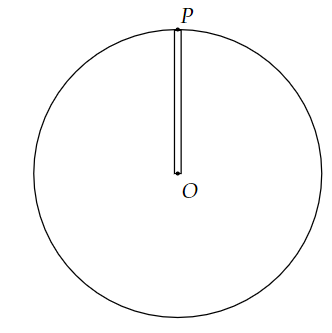
\includegraphics[width=0.31\textwidth]{imagens/q5(1).png}
            \caption{Esquema \(1\)}
        \end{figure}
        \switchcolumn
        \begin{figure}[h]
            \centering
            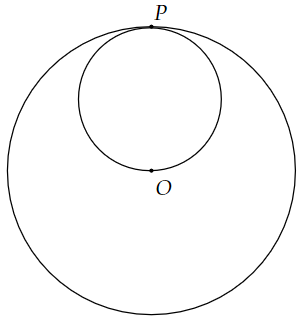
\includegraphics[width=0.3\textwidth]{imagens/q5(2).png}
            \caption{Esquema \(2\)}
        \end{figure}
    \end{paracol} 

    \begin{pssolution*}{}{}
        \begin{alternativas}
            \item A gravidade dentro de um planeta é dada por:
            \[\oint\mathbf{g}\cdot d\mathbf{S} = -4\pi GM_{int}\]
            \[4\pi r^2g = -4\pi G \rho \frac{4\pi}{3}r^3\]

            Ou seja, para o caso \(1\), \(g \propto -\rho r \rightarrow g = -k\rho r\). Utilizando a Segunda Lei de Newton:
            \[F = mv\frac{dv}{dr} = -mkr\]
            Integrando:
            \[\int_0^{v_1} v'dv' =-k\rho\int_0^R rdr\]

            \[\frac{v_1^2}{2} = k\rho\frac{R^2}{2} \rightarrow \boxed{v_1 = R \sqrt{k\rho}}\]

            Seja \(\mathbf{j}\) o vetor que parte do centro do planeta até o centro da cavidade. Utilizando superposição:
            \[a = -k\rho\mathbf{r} - k(-\rho)(\mathbf{r}-\mathbf{j}) = -k\rho\mathbf{j}\]
            Ou seja, no caso \(2\), a aceleração é constante e tem módulo \(|a| = \frac{k\rho R}{2}\).
            
            Utilizando Torricelli:
            \[v_2^2 = 2aR k\rho R^2 \rightarrow \boxed{v_2 = R\sqrt{k\rho}}\]
            Logo, \(v_1/v_2 = 1\).

            \item No primeiro caso, note que temos um M.H.S., uma vez que a força é proporcional a \(r\). O tempo até atingir a parte inferior seria igual a \(1/4\) do período:
            \[\ddot{r} = -k\rho r \rightarrow \omega^2 = k\rho \rightarrow T = \frac{2\pi}{\sqrt{k\rho}} \rightarrow t_1 = \frac{T}{4} = \frac{\pi}{2\sqrt{k\rho}}\]

            No segundo caso, temos uma aceleração constante, logo:
            \[t_2 = \frac{v_2}{a_2} = \frac{2R\sqrt{k\rho}}{k\rho R} = \frac{2}{\sqrt{k\rho}}\]

            Logo, a razão \(t_1/t_2\) é dada por:
            \[\boxed{\frac{t_1}{t_2} = \frac{\pi}{4}}\]

        \end{alternativas}
    \end{pssolution*}
\end{pproblem}

\pts{5}
\begin{pproblem} Calcular as velocidades de escape em certas situações pode ser mais complicado do que parece. Um exemplo disso é calcular a velocidade de lançamento que um foguete precisa ter para chegar a determinado local.
    \\
    \textbf{Dica:} Os problemas a seguir exigem que você pense cuidadosamente no referencial mais adequado. Não subestime a questão.
    \\
    \textbf{Dados:} Um corpo pode orbitar a superfície da Terra com velocidade \(v_0 = 7,9\text{ km/s}\), a velocidade orbital da Terra em torno do Sol é \(u_0 = 29,7\text{ km/s}\), e o raio da Terra é desprezível em relação à distância Terra-Sol. Considere também que, ao deixar o campo gravitacional da Terra, a distância entre a sonda e o Sol é a mesma distância entre a Terra e o Sol.
    \begin{enumerate}[label=\textbf{\alph*)}]
        \item Qual é a menor velocidade de lançamento que um foguete precisa ter para atingir o Sol, considerando que ele dê apenas um impulso? (Para conferir, \(v = 31,8\) km/s)
        \item Qual é a menor velocidade de lançamento que um foguete precisa ter para escapar do Sistema Solar? (Para conferir, \(v = 16,7\) km/s)
        \item Como a resposta do item \textbf{a)} muda se o foguete conseguir realizar um segundo impulso muito pequeno em algum ponto de sua órbita?
    \end{enumerate}

    \begin{pssolution*}{}{}
        \begin{alternativas}
            \item Para que isso aconteça, após deixar a Terra, no referencial do Sol, a sonda deve estar parada e, consequentemente, no referencial da Terra, ela deve estar com velocidade \(-u_0\). Utilizando conservação de energia:
            \[\frac{mv^2}{2}-\frac{GM_\oplus m}{R_\oplus} = \frac{mu_0^2}{2}\]
            \[v^2 = u_0^2+\frac{2GM_\oplus}{R_\oplus}\]

            Note que a velocidade \(v_0\) também pode ser obtida igualando a aceleração centrípeta com a gravitacional:
            \[\frac{mv_0^2}{R_\oplus} = \frac{GM_\oplus m}{R_\oplus^2} \rightarrow v_0^2 = \frac{GM_\oplus}{R_\oplus}\]

            Substituindo,

            \[v^2=u_0^2+2v_0^2 \rightarrow \boxed{v = 31,8\text{ km/s}}\]

            \item Nesse caso, ao sair do campo gravitacional da Terra, no referencial do Sol, o corpo deve ter uma velocidade \(\sqrt{2}u_0\), logo, no referencial da Terra, deve possuir \((\sqrt{2}-1)u_0\). Novamente, por conservação de energia:
            
            \[\frac{mv^2}{2}-\frac{GM_\oplus m}{R_\oplus} = \frac{m(\sqrt{2}-1)^2u_0^2}{2}\]

            \[v^2 = (\sqrt{2}-1)^2u_0^2+2v_0^2 \rightarrow \boxed{v = 16,7 \text{ km/s}}\]

            \item Imagine que façamos a sonda ir para o infinito, ou seja, a lançamos com velocidade \(v=16,7\text{ km/s}\), e, após isso, damos um impulso infinitesimal na direção do Sol. Isso faz com que a sonda percorra todo o caminho de volta e, consequentemente, atinja o Sol.
        \end{alternativas}
    \end{pssolution*}
\end{pproblem}

\pts{3} % problemas da semana 115
\begin{pproblem} (Kevin Zhou) A equação dos foguetes é dada por:
    \[
    v = u\ln\left(\frac{M_0}{M}\right)
    \]
    Onde \(v\) é a velocidade do foguete, \(u\) a velocidade relativa com que o foguete ejeta combustível, \(M_0\) a massa inicial do foguete e \(M\) sua massa atual.
    \begin{enumerate}[label=\textbf{\alph*)}]
        \item Deduza a equação dos foguetes partindo da conservação do momento.
        \item Considerando \(u\) um valor fixo durante todo o percurso do foguete, qual deve ser o valor de \(u\) para que o foguete vá de \(0\) até \(v\) gastando o menor combustível possível? (Você precisará resolver numericamente para \(v/u\))
        \item Como a equação dos foguetes deve ser corrigida para uma região do espaço com um campo gravitacional, \(\mathbf{g}\), constante e apontando na direção contrária ao movimento do foguete? Considere \(\eta = dm/dt = \text{constante}\).
    \end{enumerate}

    \begin{pssolution*}{}{}
        \begin{alternativas}
            \item Considere que o foguete possui massa \(M\) e velocidade \(v\). Ele ejeta combustível a uma velocidade relativa \(u\). Seja \(dm\) a massa de gás ejetada:
            \[dp = (v-u)dm\]
            Mas, pela definição,
            \[dp = vdm + mdv\]
            Combinando essas equações:
            \[mdv = -udm\]

            Integrando,
            \[\ln m = -\frac{v}{u} + C\]

            Sabemos que quando \(m = M_0\), temos \(v = 0\), então \(C = \ln M_0\). Assim:

            \[v = u \ln\left(\frac{M_0}{M}\right)\]

            Como esperado.

            \item A energia cinética do gás é dada por:
            
            \[K_{g} =\frac{1}{2}M_gu^2 = \frac{(M_0-M)u^2}{2}\]

            Podemos encontrar uma expressão para \(M\) utilizando a equação dos foguetes:

            \[\frac{M_0}{M} = e^{v/u} \rightarrow M_0 = Me^{v/u}\]

            Voltando à fórmula anterior:
            
            \[K_g = \frac{M(e^{v/u}-1)u^2}{2}\]

            Aqui, \(M\) seria o equivalente à massa da "carcaça" do foguete.

            Para minimizar a quantidade de energia gasta com combustível, temos:

            \[\frac{dK_g}{du}=0  \rightarrow -e^{v/u}v +2u(e^{v/u}-1)=0\]

            Definindo \(x=v/u\),

            \[e^xx = 2(e^x-1) \rightarrow x = 2(1-e^{-x})\]

            Resolvendo por iteração, encontramos:

            \[x \approx 1,59 \rightarrow \boxed{u \approx \frac{v}{1,59}} \]

            \item Nesse caso, temos:
            
            \[dp = (v-u)dm - mgdt = mdv +vdm\]
            \[\frac{dm}{m} = -\frac{dv}{u} - \frac{g}{u}dt\]

            Integrando,

            \[\ln\left(\frac{M}{M_0}\right) = -\frac{v}{u} - \frac{gt}{u}\]

            Como \(\eta\) é constante, \(M = M_0 -\eta t \rightarrow t = (M_0-M)/\eta\).

            \[\ln\left(\frac{M}{M_0}\right) = -\frac{v}{u} - \frac{g}{u\eta}(M_0-M)\]

            Resolvendo para \(v\),

            \[\boxed{v = u\ln\left(\frac{M_0}{M}\right)-\frac{g}{\eta}(M_0-M)}\]
        \end{alternativas}
    \end{pssolution*}
\end{pproblem}  

\pts{4}
\begin{pproblem} Um dos propelentes mais comuns em foguetes é uma mistura de hidrogênio líquido com oxigênio líquido. Quando começa a queimar, a seguinte reação química ocorre:
    \[
    2H_2 + O_2 \rightarrow 2H_2O
    \] 
    Para cada mol de hidrogênio, esta reação libera \(241,8 \text{ kJ}\) de energia. Ao longo da questão, suponha que toda essa energia seja utilizada para mover o foguete.
    \begin{enumerate}[label=\textbf{\alph*)}]
        \item Uma expedição espacial deseja ser feita de tal maneira que é necessário realizar uma transferência de Hohmann para lançar um foguete da Terra para Marte. Calcule a variação de velocidade total \(\Delta v\) necessária para realizar essa manobra.
        \item A partir do \(\Delta v\) calculado anteriormente, estime quantas toneladas de propelente devem ser utilizadas para realizar tal manobra para um foguete que ejeta propelente com velocidade \(u = 3,0\) km/s e carcaça com massa \(M = 140\cdot10^3\) kg.
    \end{enumerate}
    \begin{pssolution*}{}{}
        \begin{alternativas}
            \item Para o primeiro impulso, temos:
            \[v_{0,1}^2=\frac{GM}{R_T}\]
            \[v_{f,1}^2 = GM\left(\frac{2}{R_T}-\frac{1}{a}\right)\]
            A órbita de transferência possui \(a=(R_T+R_M)/2\),
            \[v_{f,1}^2 = \frac{2GM}{R_T}\left(\frac{R_M}{R_T+R_M}\right)\]

            Já no segundo impulso,
            \[v_{0,2}^2 = GM\left(\frac{2}{R_M}-\frac{1}{a}\right) = \frac{2GM}{R_M}\left(\frac{R_T}{R_T+R_M}\right)\]

            \[v_{f,2}^2 = \frac{GM}{R_M}\]

            Sendo \(\Delta v = \Delta v_1 + \Delta v_2 = (v_{f,1}-v_{0,1})+(v_{f,2}-v_{0,1})\), podemos equacionar:

            \[\boxed{\Delta v = \sqrt{\frac{2GM}{R_T}\left(\frac{R_M}{R_T+R_M}\right)}-\sqrt{\frac{GM}{R_T}} + \sqrt{\frac{GM}{R_M}} - \sqrt{\frac{2GM}{R_M}\left(\frac{R_T}{R_T+R_M}\right)}}\]
            
            Utilizando \(M = M_\odot = 2\cdot10^{30}\) kg, \(R_M = 1,5\) UA e \(R_T = 1\) UA, encontramos o valor numérico de \(\Delta v \approx 5,42 \) km/s.

            \item Utilizando a equação dos foguetes, temos:
            
            \[v = u\ln\left(\frac{M_0}{M}\right) \rightarrow \frac{M_0}{M}  = 1+ \frac{\mu}{M}= e^{v/u}\]

            Onde \(\mu\) é a massa de gás.

            \[\boxed{\mu = M(e^{v/u}-1) \approx 7,12 \cdot 10^5 \text{ kg}}\]

            O que é condizente com a realidade, uma vez que a massa do combustível é \(\approx 83\%\) da massa total do foguete.
        \end{alternativas}
    \end{pssolution*}
\end{pproblem}

\pts{3} % problemas da semana 115
\begin{pproblem} Marisso estava estudando um sistema binário com inclinação \(i\). Ele conseguiu descobrir que o maior redshift vindo da estrela \(1\) era \(z_1\). Sabendo disso, ache uma expressão para a massa da estrela \(2\), \(m_2\), deixe sua resposta em função de \(z_1\), do período do binário \(P\), da inclinação \(i\), da razão entre as massas \(\lambda  = m_2/m_1\) e de constantes fundamentais. Considere as órbitas circulares.
    \begin{pssolution*}{}{}
        A velocidade com que \(1\) orbita o CM é:

        \[v_1 = \frac{2\pi a_1}{P}\]

        Pela geometria, a velocidade radial é \(v_{r,1}=v_1\sin i\), com isso:

        \[z_1 \approx \frac{v_{r,1}}{c} = \frac{2\pi a_1\sin i}{Pc}\]

        Do teorema do centro de massa:

        \[m_1a_1=m_2a_2 \rightarrow a_2 = \frac{a_1}{\lambda}\]

        Utilizando a terceira Lei de Kepler:

        \[\frac{(a_1+a_2)^3}{P^2} = \frac{G(m_1+m_2)}{4\pi^2}\]

        \[\frac{a_1^3(1+1/\lambda)^3}{P^2} = \frac{Gm_2(1+1/\lambda)}{4\pi^2}\]

        Isolando \(m_2\):

        \[m_2 = \frac{4\pi^2a_1^3(1+1/\lambda)^2}{GP^2}\]

        \(a_1\) pode ser obtido avaliando a fórmula do redshift, \(a_1 = Pcz_1/2\pi\sin i\):

        \[m_2 = \frac{4\pi^2}{GP^2}\left(\frac{z_1Pc}{2\pi\sin i}\right)^3(1+1/\lambda)^2\]

        Por fim, simplificando:

        \[\boxed{m_2 = \frac{z_1^3c^3P}{2\pi G \sin^3i}(1+1/\lambda)^2}\]
    \end{pssolution*}
\end{pproblem}

\pts{2}
\begin{pproblem} Qual é a razão entre \(a)\) as forças gravitacionais causadas pelo Sol e pela Lua na superfície da Terra? E \(b)\) das forças de maré causadas pelo mesmo?
    \begin{pssolution*}{}{}
        \begin{alternativas}
            \item A força gravitacional tem a forma:
            \[F_G = \frac{GMm}{d^2}\]

            Assim,

            \[\frac{F_\odot}{F_L} = \frac{M_\odot}{M_L}\left(\frac{d_{T-L}}{d_{T-\odot}}\right)^2 \boxed{\approx 178,33}\]

            \item Para as forças de maré, temos:
            
            \[F_M \propto \frac{m}{d^3}\]

            \[\therefore \frac{F_\odot}{F_L} = \frac{M_\odot}{M_L}\left(\frac{d_{T-L}}{d_{T-\odot}}\right)^3 \boxed{\approx 0,456}\]

        \end{alternativas}
    \end{pssolution*}
\end{pproblem}

\pts{4}
\begin{pproblem} (Morin 7.7) Uma partícula de massa \(m\) viaja em uma órbita hiperbólica com uma massa \(M\) fixa em um dos focos. A velocidade no infinito é \(v_0\) e o parâmetro de impacto é \(b\).
    \begin{alternativas}
    \item Mostre que o ângulo de desvio da partícula é dado por:
    \[
    \phi = \pi-2\tan^{-1}(\gamma b)
    \]
    Onde \(\gamma \equiv v_0^2/GM\).
    \item Sendo \(d\sigma\) a seção transversal da partícula (medida quando a mesma se encontra no infinito) que é defletida em um ângulo sólido de tamanho \(d\Omega\). Mostre que:
    \[
    \frac{d\sigma}{d\Omega} = \frac{1}{4\gamma^2\sin^4(\phi/2)}
    \] 
    A título de curiosidade, essa quantidade é chamada de \textit{seção transversal diferencial}.
    \end{alternativas}

    \begin{pssolution*}{}{}
        \begin{alternativas}
            \item O esquema da situação é o seguinte:
            
            \begin{figure}[H]
                \centering
                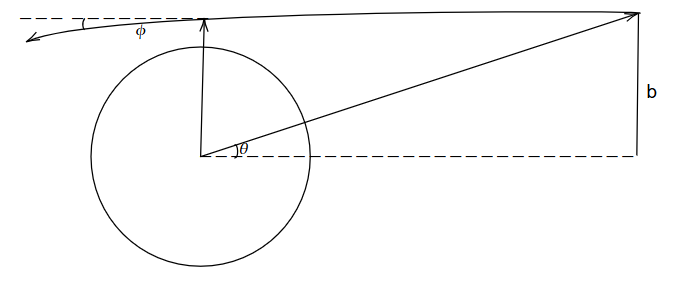
\includegraphics[width=0.87\linewidth]{imagens/orbita hiperbolica esquema 1.png}
                \caption{Esquema da Órbita Hiperbólica}
                \label{fig.1}
            \end{figure}

            Para achar o ângulo de desvio \(\phi\), vamos usar o teorema do Impulso, considerando as componentes horizontais e verticais da força de atração:

            \[F_x = -\frac{GMm}{r^2}\cos\theta, \ \ F_y = -\frac{GMm}{r^2}\sin\theta\]

            O teorema do Impulso nos diz que:
            \[\int F_i dt = \Delta p\]

            Onde \(p_i\) é o momento da partícula na direção \(i\).

            No eixo \(x\), temos:

            \[-\int \frac{GMm}{r^2}\cos\theta dt = \Delta p_x \]

            Note que integrar com relação ao tempo deixa as coisas inconvenientes, pois descobrir como \(\theta\) e \(r\) variam no tempo é algo complicado. Por isso, vamos recorrer à definição de momento angular. Utilizando que \(L = mr^2d\theta/dt\), temos:

            \[dt = \frac{mr^2}{L}d\theta\]

            Substituindo esse valor na nossa integral:
            \[-\int \frac{GMm^2}{L}\cos\theta d\theta = \Delta p_x\]

            Perceba que nossa integral vai de \(\theta = 0\), situação no infinito, até \(\theta = \pi - \phi\), situação no infinito após o desvio. Assim:

            \[-\frac{GMm^2}{L}\int_0^{\pi-\phi}\cos\theta d\theta = -\frac{GMm^2}{L}\sin\theta\big|_0^{\pi-\phi} = -\frac{GMm^2}{L}\sin(\pi-\phi) = \Delta p_x\]

            Analogamente para \(y\):

            \[-\frac{GMm^2}{L}\int_0^{\pi-\phi}\sin\theta d\theta = \Delta p_y\]
            \[=\frac{GMm^2}{L}\cos\theta\big|_0^{\pi-\phi} \equiv -\frac{GMm^2}{L}(1-\cos(\pi-\phi)) = \Delta p_y\]
        
            Note também que \(\Delta p_x = m(v_{f,x}-v_0), \ \Delta p_y = m(v_{f,y}-0)\). Podemos achar também uma relação de \(\phi\) com as velocidades e, por pura geometria, obtemos:
            \[\tan\phi =-\frac{v_{f,y}}{v_{f,x}}\]
            Como só há forças centrais, \(L\) é um valor constante, e da situação inicial, o mesmo vale \(L = mbv_0\). Agora, indo para as contas:

            \[-\frac{GM}{bv_0}\sin(\pi-\phi) = v_{f,x}-v_0, \ \ -\frac{GM}{bv_0}(1-\cos(\pi-\phi))=v_y\]
            
            Com essas duas equações, obtemos:

            \[\frac{v_{f,y}}{v_{f_x}}= -\frac{GM(1-\cos(\pi-\phi))}{bv_0^2-GM\sin(\pi-\phi)}\]

            Ou seja:

            \[\tan\phi = \frac{GM(1-\cos(\pi-\phi))}{bv_0^2-GM\sin(\pi-\phi)}\]

            Resolvendo para \(\phi\), obtemos o resultado esperado. Uma outra maneira de realizar a mesma questão é pensar puramente na geometria da situação:
            \begin{figure}[H]
                \centering
                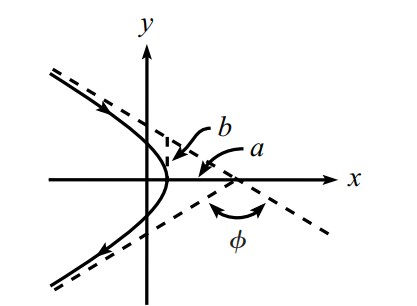
\includegraphics[width=0.7\linewidth]{imagens/morin hiperbole.png}
                \caption{Fonte: Morin 7.7}
            \end{figure}

            Aqui, é evidente que:

            \[\phi = \pi - 2\tan^{-1}\left(\frac{b}{a}\right)\]

            Onde \(b\) é o parâmetro de impacto e \(a\) o semi-eixo da hipérbole. Do conhecimento de cônicas, temos:
            \[\frac{b}{a} = \sqrt{e^2-1} = \sqrt\frac{2EL^2}{m(GMm)^2} = \frac{v_0^2b}{GM} \equiv \gamma b\]

            Em ambas as maneiras, chegamos no mesmo resultado:

            \[\boxed{\phi = \pi - \tan^{-1}(\gamma b)}\]

            Como desejado.

            \item Considere um anel de espessura \(db\) e raio \(b\). Agora, considere uma esfera bem grande, com centro em \(M\). Qualquer partícula que passar pela seção transversal do anel de raio \(b\) irá atingir essa esfera fazendo um ângulo \(\phi\) com o eixo \(x\), com uma separação angular \(d\phi\). Usando que \(d\cot x/dx = -1/\sin^2x\), temos:
            
            \[\big|\frac{db}{d\phi}\big| = \frac{1}{2\gamma \sin^2(\phi/2)}\]

            A área de seção transversal é dada por \(d\sigma = 2\pi bdb\) e o ângulo sólido de uma esfera é dado por \(d\Omega = 2\pi \sin\phi d\phi\). Portanto:

            \[\frac{d\sigma}{d\Omega} = \frac{2\pi b}{2\pi \sin \phi}\frac{db}{d\phi} = \left(\frac{(1/\gamma)\cot(\phi/2)}{2\sin(\phi/2)\cos(\phi/2)}\right)\left(\frac{1}{2\gamma\sin^2(\phi/2)}\right)\]

            \[\boxed{\frac{d\sigma}{d\Omega} = \frac{1}{4\gamma^2\sin^4(\phi/2)}}\]
        \end{alternativas}            
    \end{pssolution*}
\end{pproblem}

\begin{psidea}{}{}
    Em certas questões, é válida a utilização de vetores. Um exemplo é a questão abaixo. Para facilitar, na parte de encontrar a inclinação da órbita, observe a seguinte imagem:

    \begin{figure}[H]
        \centering
        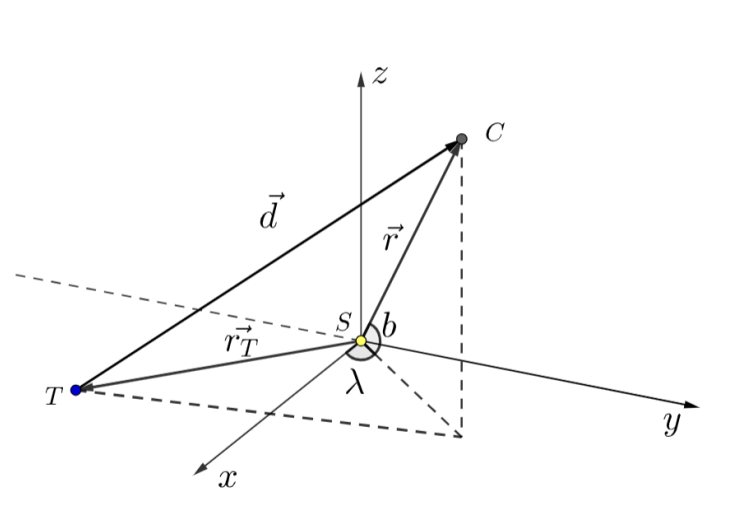
\includegraphics[width=0.7\linewidth]{imagens/vetores ecliptica.png}
        \caption{Vetores}
    \end{figure}

    Aqui, \(C\) representa um corpo, \(T\) a Terra e \(S\) o Sol. Os ângulos \(\lambda\) e \(b\) denotam, respectivamente, a longitude e a latitude eclíptica. \(\vec{r}\) é o vetor entre o Sol e o corpo, \(\vec{r}_T\) o vetor entre o Sol e a Terra, e \(\vec{d}\) o vetor entre a Terra e o corpo.
    Pela figura,

    \[\vec{r} = r(\cos b\cos\lambda \hat{x}+ \cos b \sin\lambda \hat{y} + \sin b \hat{z})\]

    \[\vec{r}_T = r_T(\cos(\omega_\oplus t)\hat{x}+\sin(\omega_\oplus t)\hat{y})\]

    Assim, \(\vec{d}=\vec{r}-\vec{r}_T\):

    \[
    \vec{d} = \big(r \cos b \cos \lambda - r_T \cos (\omega_\oplus t)\big) \hat{x} 
    + \big(r \cos b \sin \lambda - r_T \sin (\omega_\oplus t)\big) \hat{y} 
    + r \sin b \, \hat{z}
    \]

    Calculando o módulo do vetor \(\vec{d}\), obtemos que:

    \[
    d = |\vec{d}| = \sqrt{r_T^2 + r^2 - 2 r_T r \cos b \cos (\lambda - \omega_\oplus t)}
    \]

    Portanto:

    \[
    \boxed{\cos b \cos (\lambda - \omega_\oplus t) = \frac{r_T^2 + r^2 - d^2}{2 r_T r}}
    \]
\end{psidea}

\pts{5}
\begin{pproblem}(Lista \(1\) - Vinhedo 2024) 
    CR4b-2023 é uma sonda em órbita heliocêntrica que foi construída e lançada em 2023 pelo jovem prodígio Caranguejo. O objetivo da sonda era estudar as tempestades solares e captar dados para que Caranguejo analisasse em seu observatório no Espírito Santo. CR4b-2023, porém, durante uma de suas expedições ao Sol, foi atingida por uma tempestade solar e sofreu uma danificação grave. Devido a isso, a sonda se desorientou e, assim, teve todos os seus parâmetros orbitais alterados, de maneira que Caranguejo não soubesse mais sua localização.

    Visando rastrear a posição de CR4b-2023 novamente, Caranguejo utilizou-se de seu observatório para coletar os valores das separações angulares \(\Delta\phi\) entre a sonda e o Sol e os valores do diâmetro angular \(\theta_S\) da sonda, tudo em função do tempo \(t\). A tabela obtida por Caranguejo pode ser vista abaixo.

    \begin{table}[H]
        \centering
        \begin{tabular}{|c|c|c|}
            \hline
            \(\Delta\phi\) (Graus) & \(\theta_S\) (mas) & \(t\) (Dias) \\
            \hline
            0,000 & 99,27 & 0,00 \\
            4,889 & 103,67 & 1,79 \\
            17,354 & 104,72 & 7,43 \\
            29,015 & 93,06 & 20,62 \\
            27,793 & 81,18 & 25,41 \\
            13,460 & 79,77 & 45,98 \\
            11,539 & 77,97 & 51,61 \\
            2,466 & 76,44 & 54,53 \\
            2,656 & 74,84 & 55,31 \\
            7,177 & 73,90 & 57,19 \\
            10,800 & 70,63 & 58,43 \\
            22,464 & 72,92 & 91,67 \\
            13,823 & 80,50 & 130,48 \\
            \hline
        \end{tabular}
        \caption{Valores medidos por Caranguejo}
    \end{table}

    Considere que, no momento inicial \(t_0 = 0\) em que a sonda é atingida pela tempestade solar, o Sol estava exatamente no ponto de Libra e o movimento da sonda era ascendente em relação ao plano da eclíptica. Além disso, considere que o raio da sonda, supostamente esférica, é dado por \(R = 30\) km. Para essa questão, não é necessário fazer análise de erros (apesar de ser importante tentar utilizar métodos visando diminuir erros estatísticos). Com base no que foi apresentado:

    \begin{enumerate}[label=(\alph*)]
        \item Calcule os parâmetros orbitais da órbita de CR4b-2023, ou seja, seu semi-eixo maior \(a\), excentricidade \(e\), inclinação \(i\), longitude do nodo ascendente \(\Omega\) e argumento do periélio \(\omega\). Como em todas as questões de análise de dados, você deve fornecer tabelas de dados claramente rotuladas, gráficos claramente rotulados e derivações de fórmulas suficientes para deixar claro o que você mediu e como está derivando seus resultados visando reduzir erros estatísticos.
        
        \item Considerando \((x', y', z')\) como as coordenadas de CR4b-2023 em um sistema cartesiano de mão direita em que o plano \(x'y'\) se localiza no plano da órbita da sonda, o Sol se localiza na origem, e o eixo \(x'\) aponta para o ponto vernal, escreva, em uma tabela, os valores de pelo menos 5 pontos \((x', y', z')\) distintos. Com base nos dados encontrados, esboce, em um gráfico, a órbita de CR4b-2023, indicando as coordenadas de seu centro.
        
        \item Considerando agora um novo sistema de coordenadas de mão direita \((x, y, z)\), no qual o Sol se localiza na origem, o plano \(xy\) representa o plano da eclíptica, e o eixo \(x\) aponta para o ponto vernal, escreva as coordenadas do centro da órbita de CR4b-2023. Por fim, calcule a distância \(d_{TC}\) entre o centro da órbita terrestre e o centro da órbita da sonda.
    \end{enumerate}

    \begin{pssolution*}{}{}
        \begin{alternativas}
            \item A ideia dessa parte da questão é encontrar uma relação entre os dias e a distância da sonda até o Sol. Utilizando trigonometria básica, podemos dizer que a distância da sonda até a Terra é dada por:
            \[d_{S-\oplus} = R/\tan^{-1}\left(\frac{\theta_S}{2}\right)\]
            Onde \(R\) é o raio da sonda.
            Aqui, podemos utilizar a lei dos cossenos para encontrar a relação dessa distância com a distância da sonda até o Sol. Considerando a órbita da Terra circular de raio \(d_{\odot-\oplus}\) e definindo por \(d\) a distância entre a sonda e o Sol, temos:
            \[d^2 = d_{\odot-\oplus}^2+d_{S-\oplus}^2-2d_{\odot-\oplus}d_{S-\oplus}\cos\Delta\phi\]      
            
            Com isso, podemos montar a seguinte tabela, com os valores de \(d\) em UA e os valores de \(t\) em dias.

            \[
                \begin{array}{|c|c|}
                \hline
                \text{t (Dias)} & \text{d (UA)} \\
                \hline
                0.00 &    0.17 \\
                1.79 &    0.22 \\
                7.43 &    0.34 \\
                20.62 &    0.50 \\
                25.41 &    0.49 \\
                45.98 &    0.24 \\
                51.61 &    0.22 \\
                54.53 &    0.09 \\
                55.31 &    0.12 \\
                57.19 &    0.18 \\
                58.43 &    0.27 \\
                91.67 &    0.44 \\
                130.48 &    0.25 \\
                \hline
                \end{array}
            \]

            Plotando um gráfico de \(t\) por \(d\), temos:
            
            \begin{figure}[H]
                \centering
                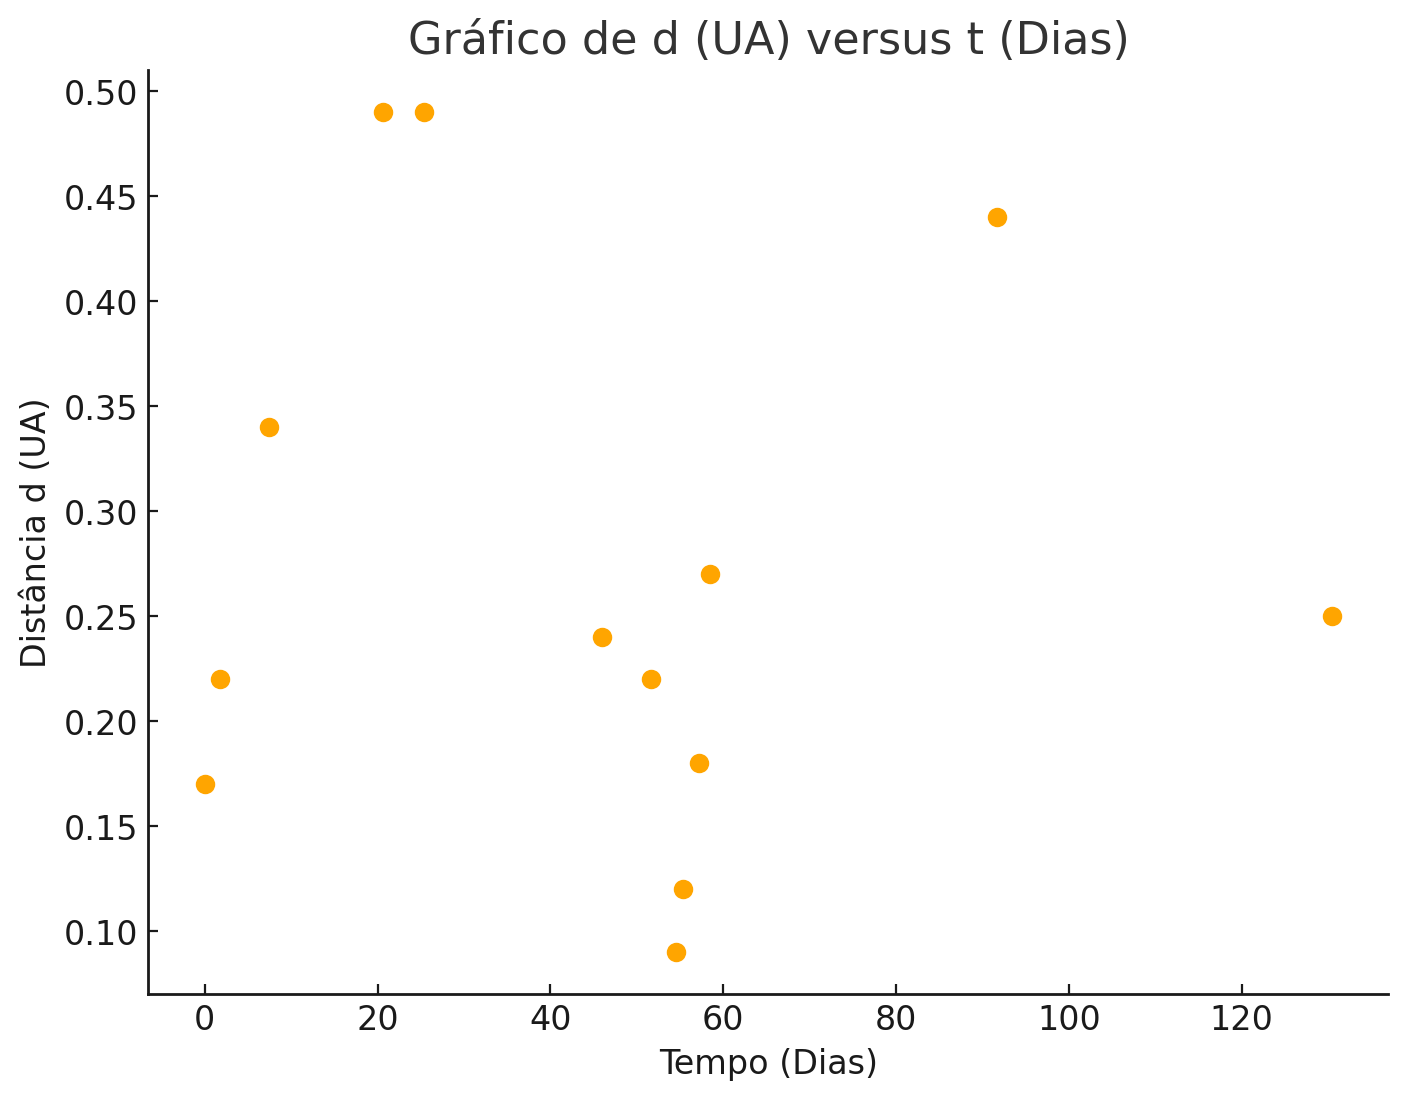
\includegraphics[width=0.85\linewidth]{imagens/graficoorbita.png}
            \end{figure}

            Agora, vamos colocar a mão na massa e achar os parâmetros requisitados: semi-eixo maior, \(a\), excentricidade, \(e\), inclinação, \(i\), longitude do nodo ascendente \(\Omega\) e argumento do periélio, \(\omega\). Os dois primeiros podem ser obtidos diretamente dos dados que analisamos até o momento.

            Analisando os dados, podemos perceber que a menor distância entre a sonda e o Sol é dada por \(a_p = 0.09\) UA e a maior distância é dada por \(a_a = 0,49\) UA. Essas distâncias devem corresponder ao periélio e ao afélio, respectivamente. Utilizando a definição:
            \[a_p = a(1-e), \ a_a=a(1+e) \rightarrow \frac{a_p}{a_a}=\frac{1-e}{1+e} \approx 0,18\]
            
            Resolvendo, obtemos \(e \approx 0,67\).

            Usando que \(a = \frac{a_p+a_a}{2}\), obtemos \(a\approx 0,30\) UA.

            Para acharmos os fatores angulares, temos que pensar um pouco mais. Começando por \(\Omega\), note que no momento inicial, em \(t=0\), a separação angular entre o Sol e a sonda é \(\Delta \phi = 0\). O enunciado nos diz que nesse momento o Sol se encontra no ponto de Libra, assim, temos que a sonda também se encontra no ponto de Libra e, como seu movimento era ascendente, temos \(\Omega = 0^\circ\).

            Para encontrar \(\omega\) e \(i\), vamos nos atentar ao seguinte triângulo esférico:

            \begin{figure}[H]
                \centering
                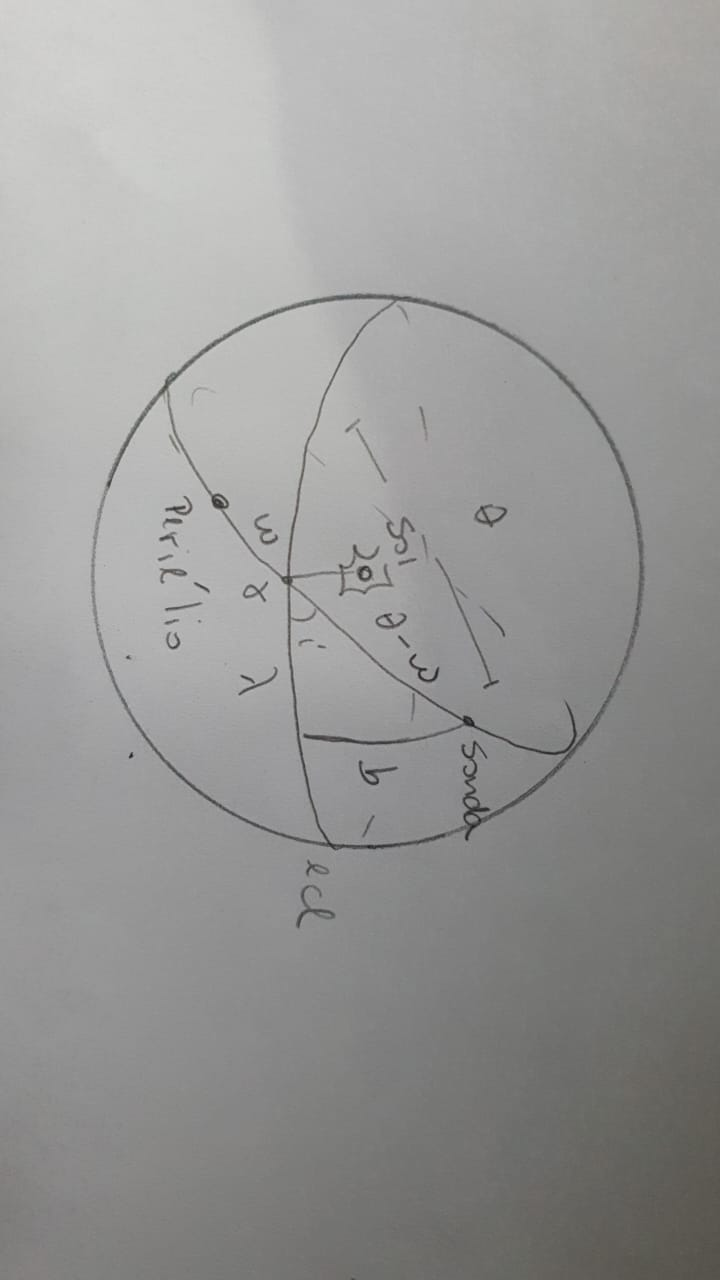
\includegraphics[angle=90, width=0.8\textwidth]{imagens/trigesfericoorbita.jpg}
                \caption{Esquema}
            \end{figure}

            Da forma polar da elipse, \(r=\frac{a(1-e^2)}{1+e\cos\theta}\), onde \(\theta\) é a anomalia verdadeira da órbita, podemos encontrar \(\omega\). Perceba que no instante inicial, \(t=0\), a sonda está exatamente no ponto de Libra, assim \(\theta = 2\pi-\omega\) conforme o esquema.

            Assim, temos:

            \[d(0) = \frac{a(1-e^2)}{1+e\cos(2\pi-\omega)}\]

            Resolvendo para \(\omega\):

            \[\omega = 2\pi-\cos^{-1}\left(\frac{a(1-e^2)}{d(0)e}-\frac{1}{e}\right) \approx 267,6^\circ \approx 270^\circ\]

            Substituindo os valores encontrados.

            Para achar a inclinação, vamos utilizar a lei dos cossenos:

            \[\cos(\theta-\omega)=\cos\lambda\cos b + \sin\lambda\sin b\cos(\pi/2) = \cos\lambda\cos b\]
            
            Note que \(\cos(\theta-\omega) \approx \cos(\theta-270^\circ) = \sin \theta\).

            Reescrevendo,

            \[\cos b = \frac{\sin\theta}{\cos\lambda}\]

            Utilizando a relação obtida na ideia anterior,

            \[\cos b  = \frac{r_T^2 + r^2 - d^2}{2 r_T r\cos (\lambda - \omega_\oplus t)}\]

            Igualando essas expressões e resolvendo para \(\lambda\),

            \[\lambda = \tan^{-1} \left( 
                \frac{r_T^2 + r^2 - d^2}{2 r_T r \sin \theta \sin (\omega_\oplus t)} - \cot (\omega_\oplus t)
                \right)\]

            Onde:

            \[
            \theta = \arccos \left( \frac{a (1 - e^2)}{e r} - \frac{1}{e} \right)
            \] 
            
            Com isso, podemos fazer a seguinte tabela, com os valores de \(b\) e \(\lambda\).

            \[
            \begin{array}{|c|c|}
            \hline
            \lambda \, (\text{Graus}) & b \, (\text{Graus}) \\ \hline
            0,000     & 0,00     \\ 
            17,495    & 9,847    \\ 
            45,905    & 22,521   \\ 
            78,492    & 29,499   \\ 
            101,508   & 29,499   \\ 
            134,095   & 22,521   \\ 
            163,504   & 9,847    \\ 
            180,000   & 0,000    \\ 
            197,495   & -9,847   \\ 
            216,005   & -18,747  \\ 
            270       & -30      \\ 
            333,435   & -14,478  \\ 
            17,495    & 9,847    \\ 
            78,492    & 29,499   \\ 
            143,994   & 18,747   \\ \hline
            \end{array}
            \]

            Voltando ao triângulo esférico e utilizando a lei dos quatro elementos, temos:

            \[\cos\lambda\cos90^\circ = \sin\lambda\cot b -\sin90^\circ\cot i\]

            Simplificando:

            \[\tan b = \tan i \sin \lambda\]

            Note que isso se assemelha a uma função do tipo \(y= A + Bx\). Fazendo uma regressão linear na calculadora, encontramos \(B\approx 0,578\). De modo que \(\tan i = B\), chegamos em:

            \[\boxed{i \approx 30^\circ}\]

        \item Como o Sol se localiza na origem, os valores de \(x'\) e \(y'\) podem ser calculados por:
            \[
            x' = r \sin \theta
            \]
            e
            \[
            y' = -r \cos \theta
            \]

            Escrevendo em uma tabela cinco valores diferentes de \(x'\) e \(y'\), obtemos que:

            \[
            \text{Tabela 7: Valores de \(x'\) e \(y'\)}
            \]

            \[
            \begin{array}{|c|c|}
            \hline
            x'\text{ UA} & y'\text{ UA} \\ \hline
            0,167 & 0,000 \\ \hline
            0,084 & 0,478 \\ \hline
            -0,219 & 0,261 \\ \hline
            -0,203 & 0,074 \\ \hline
            0,000 & -0,100 \\ \hline
            \end{array}
            \]

            Perceba que quaisquer valores, desde que corretos, de \(x'\) e \(y'\) podem ser utilizados. Além do mais, é importante aumentar o espaçamento entre os valores de \(x'\) e \(y'\) visando diminuir os erros associados ao esboço da órbita. Com base nisso, podemos plotar o gráfico:

            \begin{figure}[H]
                \centering
                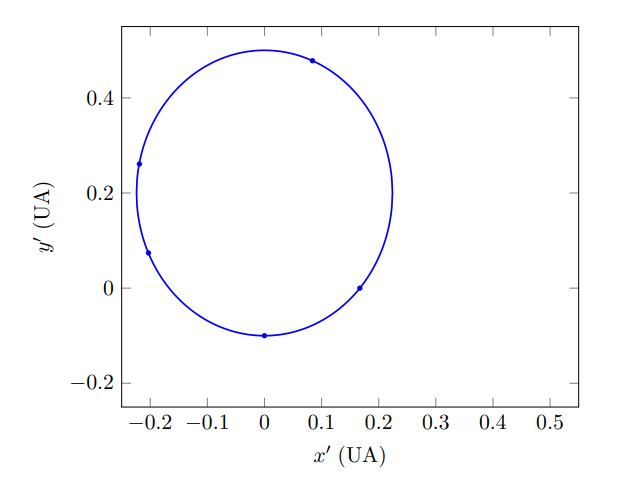
\includegraphics[width=0.7\linewidth]{imagens/graforbt.png}  
                \caption{Gráfico da órbita} 
            \end{figure}

            Observando o gráfico, vemos que as coordenadas \((x', y', z')\) do centro da elipse são \(\boxed{(0;\ 0,2; \ 0)}\).

        \item Aqui, vamos utilizar uma matriz de rotação em torno do eixo \(x\), dada por:
        
            \[
            \begin{pmatrix}
            x \\
            y \\
            z
            \end{pmatrix}
            =
            \begin{pmatrix}
            1 & 0 & 0 \\
            0 & \cos \alpha & \sin \alpha \\
            0 & -\sin \alpha & \cos \alpha
            \end{pmatrix}
            \begin{pmatrix}
            x' \\
            y' \\
            z'
            \end{pmatrix}
            \] 

            Para \(\alpha=i=30^\circ\):

            \[
            \begin{pmatrix}
            x \\
            y \\
            z
            \end{pmatrix}
            =
            \begin{pmatrix}
            1 & 0 & 0 \\
            0 & \cos 30^\circ & \sin 30^\circ \\
            0 & -\sin 30^\circ & \cos 30^\circ
            \end{pmatrix}
            \begin{pmatrix}
            x' \\
            y' \\
            z'
            \end{pmatrix}
            \]

            Então:
            \[
            x = x'
            \]
            \[
            y = y' \cos 30^\circ + z' \sin 30^\circ
            \]
            \[
            z = -y' \sin 30^\circ + z' \cos 30^\circ
            \]

            Substituindo os valores numéricos, obtemos que as coordenadas \((x, y, z)\) do centro de CR4b-2023 são dadas por:
            \[
            (0.000, 0.173, -0.100).
            \]

            Por fim, obtemos então que a distância entre o centro da órbita terrestre e o centro da órbita da sonda é dada por:
            \[
            d = \sqrt{\lvert x^2 + y^2 + z^2 \rvert}
            \]

            ou seja:
            \[
            \boxed{d = 0.200 \, \text{UA}}
            \]
        \end{alternativas}
    \end{pssolution*}
\end{pproblem}

\pts{5}
\begin{pproblem} (Iran Problem Set) 
    Uma partícula de massa \(m\) está orbitando um objeto massivo de massa \(M\). Mostre que o impulso necessário para fazer a órbita girar um ângulo \(\eta\) em torno de um dos focos é dado por:
    \[
    \Delta v = \frac{2\mu e}{h}\sin\left(\frac{\eta}{2}\right),
    \]
    onde:
    \begin{itemize}
        \item \(h\) é o momento angular por unidade de massa;
        \item \(\mu = GM\), sendo \(G\) a constante gravitacional.
    \end{itemize}
    \begin{pssolution*}{}{}
        Desenhando a órbita e a órbita rotacionada:

        \begin{figure}[H]
            \centering
            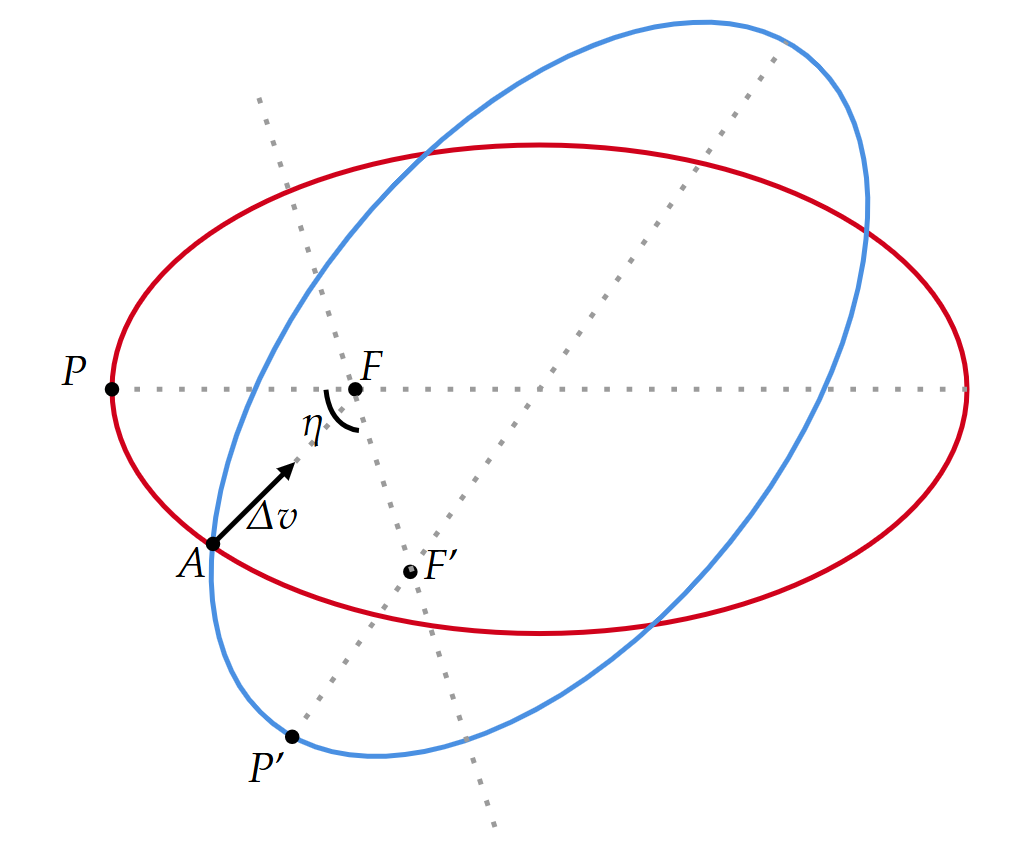
\includegraphics[width=0.7\linewidth]{imagens/esquemarotorb.png}
            \caption{Esquema da órbita rotacionada.}
        \end{figure}

        Perceba que o impulso só pode ser realizado nos pontos de interseção das duas órbitas e deve ser radial, uma vez que o momento angular deve continuar constante, a fim de manter a órbita idêntica. Vamos definir por \(X\) um ponto na órbita antes do impulso e \(X'\) um ponto na órbita após a rotação.

        Vamos às seguintes definições: \(F\) é o foco, \(P\) é o periélio da órbita, e \(A\) é o ponto de interseção onde é realizado o impulso.

        Por simetria, note que os ângulos \(AFP\) e \(AFF'\) são iguais e, portanto, têm valor \(\eta/2\).

        Como as duas órbitas possuem o mesmo momento angular, a velocidade tangencial no ponto \(A\) deve ser equivalente para ambas as órbitas. Além disso, podemos perceber que o ponto \(A\) possui anomalia verdadeira \(\theta = \eta/2\), o que garante que o módulo da velocidade também seja o mesmo para ambas as órbitas.

        \begin{figure}[H]
            \centering
            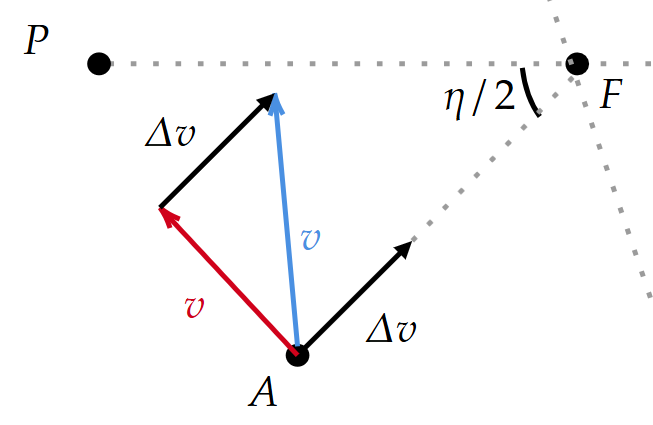
\includegraphics[width=0.7\linewidth]{imagens/rotorbt1.png}
            \caption{Vetores de velocidade.}
        \end{figure}

        A única maneira de isso ser possível seria se o impulso radial fosse dado por \(\Delta v = 2v_r\), onde \(v_r\) é a velocidade radial imediatamente antes do impulso.

        É claro que \(v_r^2 = v^2 - v_t^2\), onde \(v_t\) é a velocidade tangencial. Partindo de definições básicas:

        \[
        h^2 = \mu a (1 - e^2), \quad r = \frac{a(1 - e^2)}{1 - e\cos\theta}, \quad v_t = \frac{h}{r}, \quad v^2 = \mu \left(\frac{2}{r} - \frac{1}{a}\right).
        \]

        Trabalhando com essas equações, chegamos a:

        \[
        v^2 = \frac{\mu^2}{h^2}(1 + 2e\cos\theta + e^2), \quad v_t^2 = \frac{\mu^2}{h^2}(1 + e\cos\theta)^2.
        \]

        Por fim, substituindo em \(v_r^2 = v^2 - v_t^2\), obtemos:

        \[
        v_r^2 = \frac{\mu^2}{h^2}(e^2 - e^2\cos^2\theta) \equiv \frac{\mu^2e^2}{h^2}\sin^2\theta.
        \]

        Substituindo \(\Delta v = 2v_r\) e \(\theta = \eta/2\), chegamos ao resultado desejado:

        \[
        \boxed{\Delta v = \frac{2\mu e}{h}\sin\left(\frac{\eta}{2}\right) \blacksquare}
        \]
    \end{pssolution*}
\end{pproblem}


\pts{3}
\begin{pproblem}
    Nessa questão, vamos estudar um modelo simplificado para o efeito que confirmou a Teoria da Relatividade Geral de Einstein: as lentes gravitacionais. A presença de um corpo massivo curva o espaço-tempo, fazendo com que estrelas possam servir como lentes no espaço. Alguns telescópios, como o JWST, utilizam esse efeito para conseguir fotografar aglomerados de galáxias muito distantes. Uma das fotos tiradas pelo JWST de uma lente gravitacional pode ser vista a seguir:
    \begin{figure}[H]
        \centering
        \includegraphics[width=0.7\linewidth]{imagens/fotoJWSTeinstenring.png}
        \caption{Fonte: National Geographic}
    \end{figure} 

    Um esquema simplificado das lentes gravitacionais pode ser observado a seguir. Esse "círculo" é conhecido como Anel de Einstein.
    \begin{figure}[H]
        \centering
        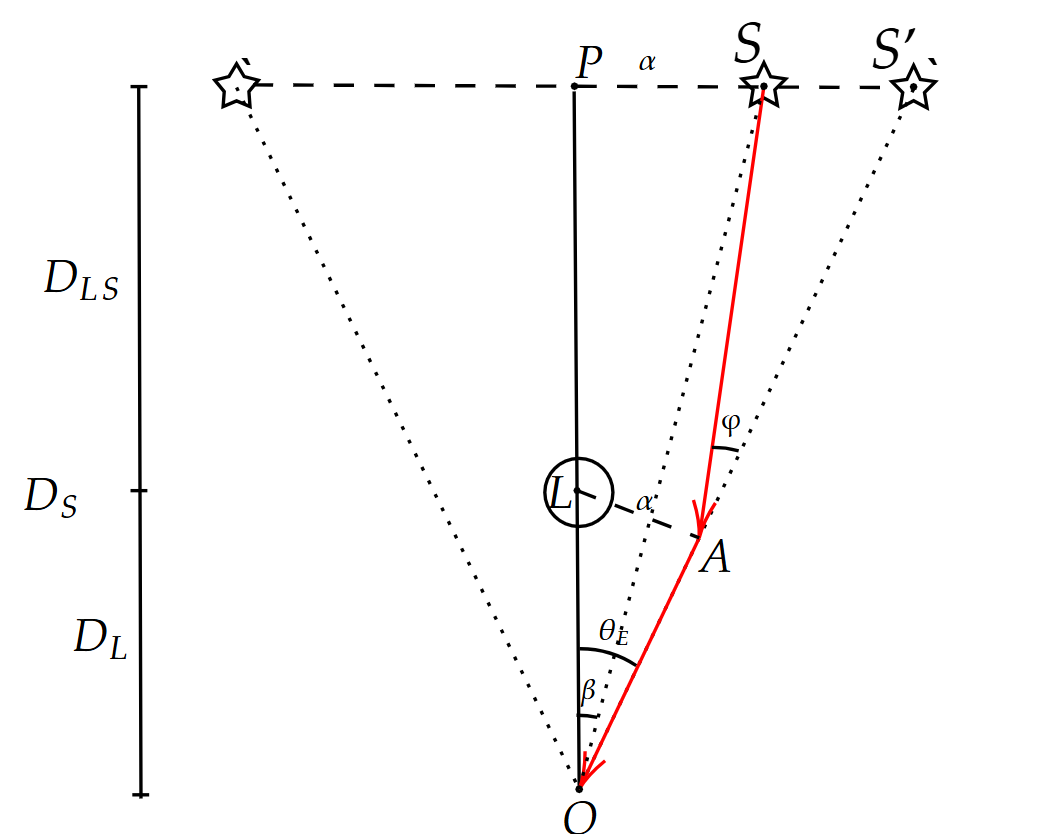
\includegraphics[width=0.9\linewidth]{imagens/anelE.png}
        \caption{Esquema da lente gravitacional}
    \end{figure}
    No esquema, o ponto \(O\) representa o observador, \(L\) o corpo massivo que atua como uma lente, \(S\) a posição real do objeto observado e \(S'\) sua posição aparente, \(\alpha\) é o parâmetro de impacto, \(\beta\) a separação angular entre o corpo observado e a lente, \(\theta_E\) o raio angular do anel de Einstein, \(\varphi\) o desvio angular causado por um corpo massivo. A distância \(\overline{OL}\) vale \(D_L\) e a distância \(\overline{OP}\) vale \(D_S\), de modo que \(D_S-D_L = D_{LS}\).

    Todos os ângulos são muito pequenos, de modo que \(\sin x \approx \tan x \approx x\). Além disso, por estarem no infinito, as retas \(\overline{OP}\), \(\overline{OS}\) e \(\overline{OS'}\) podem ser aproximadas como paralelas.

    É um resultado conhecido da Teoria da Relatividade Geral que o desvio da luz causado por um corpo massivo é dado por:
    \[\varphi = \frac{4GM}{\alpha c^2}\]
    \begin{alternativas}
        \item No limite em que \(\lim_{\alpha \rightarrow 0}\), encontre uma expressão para \(\theta_E\) em função das demais distâncias e ângulos fornecidos.
    
        \item O telescópio JWST obtém imagens no infravermelho, de comprimento de onda \(\lambda_{IV}\). Quão grande deve ser seu diâmetro para que ele possa resolver um anel de Einstein?
    \end{alternativas}

    \begin{pssolution*}{}{}
        \begin{alternativas}
            \item Note que, quando \(\alpha \rightarrow 0\), \(\overline{PL}=\overline{AS}=D_{LS}\). Utilizando \(\tan\theta = \sin\theta=\theta\), temos:
            
            \[(1)\ \overline{PS} = D_S\beta = \alpha, \ \ (2)\ \overline{SS'} = D_{SL}\varphi, \ \ (3)\ \overline{PS'} = D_S\theta_E,\] 
            \[(4)\ \overline{OL} = D_L = \overline{LA}/\theta_E = \alpha\theta_E, \ \ (5)\ \overline{LA}=\overline{PS}, \ \ (6)\ \overline{PS'} = \overline{PS}+\overline{SS'}\]

            Substituindo \((1), \ (2), \ (3)\) em \((6)\), 

            \[D_S\theta_E=D_S\beta+(D_S-D_L)\varphi\]

            \[\theta_E-\beta = \frac{D_S-D_L}{D_S}\varphi\]

            Substituindo o valor de \(\varphi\):

            \[\theta_E-\beta = \frac{D_S-D_L}{D_S}\frac{4GM}{\alpha c^2}\]

            Utilizando \((4)\), temos \(\alpha=D_L\theta_E\) e substituindo na nossa equação:

            \[\theta_E-\beta = \frac{D_S-D_L}{D_S}\frac{4GM}{D_L\theta_E c^2}\]

            \[\theta_E^2-\beta\theta_E = \frac{D_S-D_L}{D_S}\frac{4GM}{c^2}\]

            O limite de \(\alpha\rightarrow 0\) implica que \(\beta\rightarrow 0\), assim:

            \[\boxed{\theta_E=\sqrt{\frac{D_S-D_L}{D_S}\frac{4GM}{c^2}}}\]

            \item Utilizando o critério de Rayleigh \(\theta = R\frac{\lambda}{D}\), onde \(R\approx 1,22\). Isolando \(D\) e substituindo \(\theta = \theta_E\):
            
            \[\boxed{D =\sqrt{\frac{c^2R^2\lambda_{IV}^2}{4GM}\frac{D_S}{D_S-D_L}}}\]
        \end{alternativas}
    \end{pssolution*}
\end{pproblem}

\pts{4}
\begin{pproblem}
    Neste exercício, vamos estudar propriedades da excentricidade das órbitas e entender como ela se relaciona com a energia e o momento angular. Denotando \(\mu = GM\) e \(h=L/m\), faça o que se pede nos itens a seguir.
    \begin{center}
        \textbf{Parte I: O vetor excentricidade}
    \end{center}
    \begin{alternativas}
        \item Escreva uma expressão para a segunda lei de Newton no formato vetorial para um corpo de massa \(m\) orbitando um corpo de massa \(M\) a uma distância \(r\).
        
        \item Faça o produto vetorial da sua expressão por \(\mathbf{h}\) e prove que:
        
        \[\frac{d}{dt}(\dot{\mathbf{r}}\times \mathbf{h}) = \frac{\mu}{r}\mathbf{v} - \frac{\mu \dot{r}}{r^2}\mathbf{r}\]

        Onde \(\dot{\mathbf{r}}\) representa a velocidade radial e \(\mathbf{v}\) a velocidade.

        \item Podemos escrever o lado direito da equação anterior como:
        \[\frac{d}{dt}\left(A\mathbf{r}\right)\]

        Encontre o valor de \(A\).

        \item Integre os dois lados da igualdade encontrada e faça a multiplicação escalar de ambos os lados por \(\mathbf{r}\). Após isso, resolva para \(r\). O seu resultado deve ser bem parecido com o previsto somente pela geometria:
        \[r = \frac{p}{1+e\cos\theta}\]

        Encontre os valores de \(p\) e \(e\). \textbf{Não esqueça da constante de integração. Suas respostas podem depender dela.}

        \item No item anterior, \(e\) é a excentricidade da órbita. Voltando à equação obtida inicialmente no item \(c\), após a integração, ache uma forma de expressar \(\mathbf{e}\), como sendo um vetor de módulo \(e\) e que aponta diretamente para o corpo orbitado.
        
        \item Prove que a relação encontrada no item anterior pode ser escrita como:
        \[\mu \mathbf{e} = (v^2-\frac{\mu}{r})\mathbf{r} - (\mathbf{r}\cdot\mathbf{v})\mathbf{v}\]

        Para onde esse vetor aponta?
    \end{alternativas}
    \begin{center}
        \textbf{Parte II: Determinando elementos orbitais a partir do vetor excentricidade}     
    \end{center}
    Vamos definir o nosso sistema de coordenadas da seguinte maneira. Considere um sistema de mão direita, orientado de tal forma que o plano \(xy\) coincida com o plano equatorial e com \(\mathbf{z}\) apontando para o polo norte. Definindo o vetor nodal como \(\mathbf{n} = \mathbf{z} \times \mathbf{h}\).
    \begin{alternativas}
        \item Encontre uma expressão para \(\mathbf{h}\) em função das componentes do vetor \(\mathbf{r}\) e do vetor \(\mathbf{v}\). Após isso, encontre o vetor \(\mathbf{n}\) em função das componentes de \(\mathbf{h}\).

        \item Desenhe uma esfera celeste e represente nela: o plano do equador e uma órbita qualquer (que tenha inclinação diferente de 0). Nela, marque os seguintes ângulos: \(i\), a inclinação orbital, \(\Omega\) a longitude do nodo ascendente, \(\omega\) o argumento do periastro e \(\theta\), a anomalia verdadeira. 

        \item Encontre expressões para todos esses ângulos em função de \(\mathbf{e}\), \(\mathbf{h}\), \(\mathbf{n}\), \(\mathbf{r}\) e qualquer um dos vetores definidos no nosso sistema de coordenadas \(xyz\).
    \end{alternativas}

    \begin{pssolution*}{}{}
        \begin{center}
            \textbf{Parte I}
        \end{center}
        \begin{alternativas}
            \item Utilizando a forma vetorial da força gravitacional, temos:
            \[-\frac{GMm}{r^3}\mathbf{r} = m\ddot{\mathbf{r}} \rightarrow \boxed{\ddot{\mathbf{r}}= -\frac{\mu}{r^3}\mathbf{r}}\]

            \item Fazendo o produto vetorial dessa expressão por \(\mathbf{h}\), temos:
            
            \[\ddot{\mathbf{r}}\times \mathbf{h} = -\frac{\mu}{r^3}(\mathbf{r}\times\mathbf{h}) = \frac{\mu}{r^3}(\mathbf{h}\times\mathbf{r})\]

            Uma vez que \(\mathbf{h}\) é constante, o lado esquerdo da equação pode ser escrito como \(d(\dot{\mathbf{r}}\times \mathbf{h})/dt\). Para o lado direito, vamos escrever \(\mathbf{h} = \mathbf{r}\times \mathbf{v}\) e utilizar a regra do BAC-CAB, que diz que \((A \times B) \times C = B(A\cdot C) - C(A \cdot B)\). Desse modo:

            \[\frac{d}{dt}(\dot{\mathbf{r}}\times \mathbf{h}) = \frac{\mu}{r^3}((\mathbf{r}\times\mathbf{v})\times \mathbf{r}) = \frac{\mu}{r^3}(r^2\mathbf{v} - \mathbf{r}(\mathbf{r}\cdot \mathbf{v}))\]

            Note que \(\mathbf{r}\cdot\mathbf{v}\) é a multiplicação das componentes de \(\mathbf{r}\) e \(\mathbf{v}\) que estão na mesma direção. Assim, \(\mathbf{r}\cdot\mathbf{v} = r\dot{r}\). Substituindo na expressão anterior:

            \[\boxed{\frac{d}{dt}(\dot{\mathbf{r}}\times \mathbf{h}) = \frac{\mu}{r}\mathbf{v} - \frac{\mu \dot{r}}{r^2}\mathbf{r}}\]

            \item Abrindo a expressão fornecida pelo enunciado:
            
            \[\frac{d}{dt}(A\mathbf{r}) = \mathbf{r}\frac{d}{dt}A + A \mathbf{v}\]

            Comparando as expressões, é fácil perceber que \(\boxed{A = \mu/r}\).

            \item Utilizando as informações obtidas nos itens anteriores, temos:
            \[\frac{d}{dt}(\dot{\mathbf{r}}\times \mathbf{h}) = \mu\frac{d}{dt}\left(\frac{\mathbf{r}}{r}\right)\]

            Multiplicando ambos os lados por \(dt\) e integrando, temos:

            \[\dot{\mathbf{r}}\times\mathbf{h} = \frac{\mu}{r}\mathbf{r} + \mathbf{B}\]

            Onde \(B\) é um vetor constante de integração. Agora, fazendo o produto escalar com \(\mathbf{r}\):

            \[\mathbf{r}\cdot(\dot{\mathbf{r}}\times \mathbf{h}) = \mu r + \mathbf{r}\cdot\mathbf{B}\]

            Usando que \(a\cdot(b\times c) = (a\times b)\cdot c\) e definindo \(\nu\) como o ângulo entre \(\mathbf{r}\) e \(\mathbf{B}\), temos:

            \[h^2 = \mu r + rB\cos\nu\]

            Resolvendo para \(r\), chegamos em:

            \[r = \frac{h^2/\mu}{1+(B/\mu)\cos\nu}\]

            Assim:

            \[\boxed{p = \frac{h^2}{\mu}, \ \ \ \ e = \frac{B}{\mu}}\]

            \item Utilizando \(\mathbf{e} = \mu \mathbf{B}\) e voltando ao item \(d)\), temos:
            \[\dot{\mathbf{r}}\times \mathbf{h} = \frac{\mu}{r}\mathbf{r}+\mu \mathbf{e}\]

            Resolvendo para \(\mathbf{e}\) e notando que \(\dot{\mathbf{r}}\times\mathbf{h} = \mathbf{v}\times\mathbf{h}\), temos:

            \[\boxed{\mathbf{e} = \frac{\mathbf{v}\times\mathbf{h}}{\mu} - \frac{\mathbf{r}}{r}}\]

            \item Escrevendo \(\mathbf{h} = \mathbf{r}\times\mathbf{v}\), temos:
            \[\mathbf{e} = \frac{\mathbf{v}\times(\mathbf{r}\times\mathbf{v})}{\mu} - \frac{\mathbf{r}}{r} \]

            Multiplicando os dois lados da expressão por \(\mu\), e usando o BAC-CAB, temos:

            \[\mu\mathbf{e} = v^2\mathbf{r} - \mathbf{v}(\mathbf{v}\cdot\mathbf{r}) - \frac{\mu}{r}\mathbf{r}\]

            Reorganizando os termos:

            \[\boxed{\mu \mathbf{e} = (v^2-\frac{\mu}{r})\mathbf{r} - (\mathbf{r}\cdot\mathbf{v})\mathbf{v}}\]

            Logo, esse vetor aponta para o periastro.
        \end{alternativas}
        \begin{center}
            \textbf{Parte II: Determinando elementos orbitais a partir do vetor excentricidade}     
        \end{center}
        \begin{alternativas}
            \item O vetor $\mathbf{h}$ é definido por $\mathbf{h} = \mathbf{r}\times\mathbf{v}$. Por definição,
            
            $$\mathbf{h}=\mathbf{r}\times\mathbf{v} = 
            \begin{vmatrix}
                \hat{x} & \hat{y} & \hat{z} \\
                r_x & r_y & r_z \\
                v_x & v_y & v_z \\
            \end{vmatrix}
            = (r_yv_z - r_zv_y)\hat{x} + (r_zv_x-r_xv_z)\hat{y} + (r_xv_y-r_yv_z)\hat{z}   $$

            De maneira similar, $\mathbf{n} = \mathbf{z}\times\mathbf{h}$
            $$\mathbf{n} = 
            \begin{vmatrix}
                \hat{x} & \hat{y} & \hat{z} \\
                0 & 0 & 1 \\
                h_x & h_y & h_z \\
            \end{vmatrix}
             = -h_y\hat{x} + h_x\hat{y}$$

             \item O desenho deve se parecer com a figura a seguir:
             \begin{figure}[H]
                \centering
                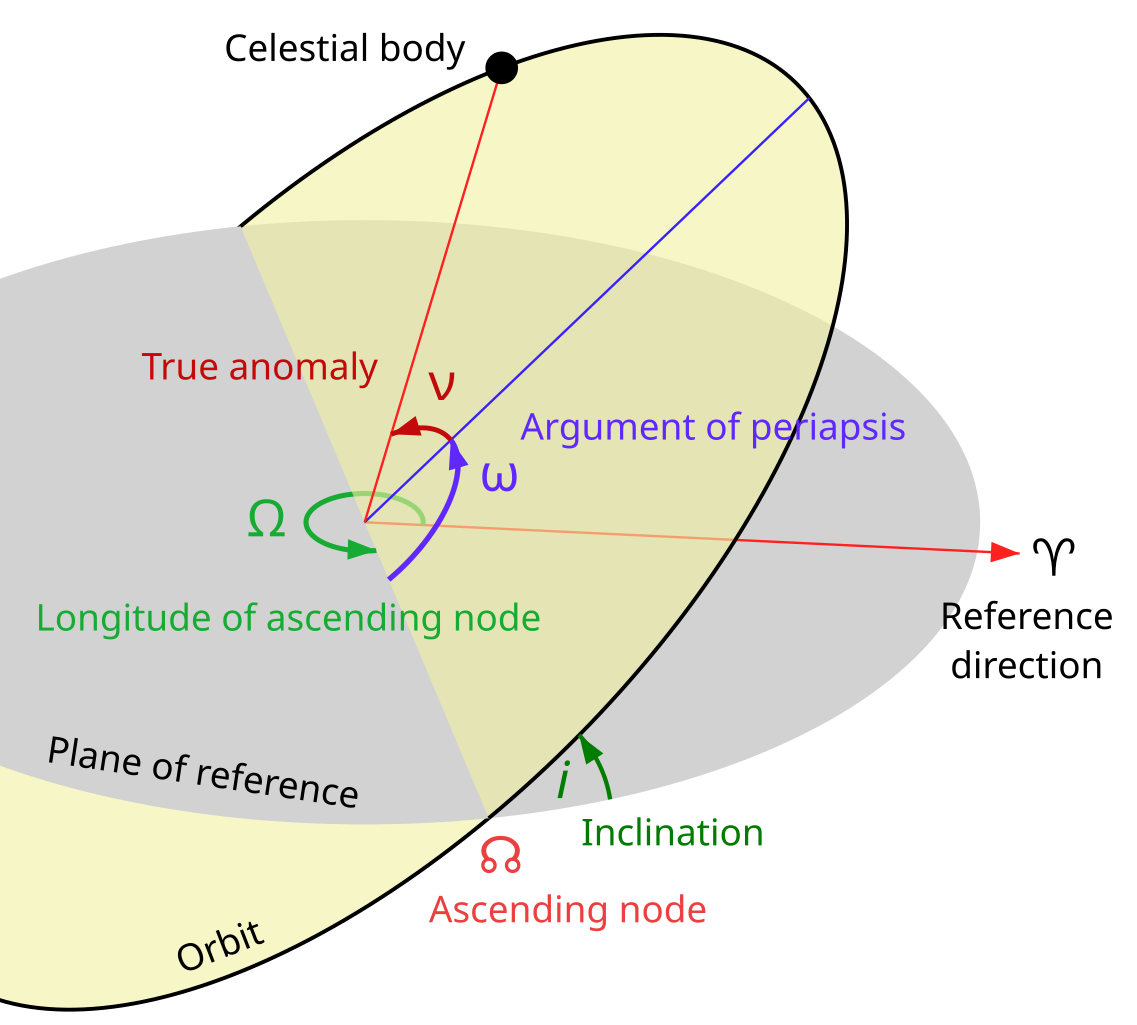
\includegraphics[width=0.7\linewidth]{imagens/elementosorbitais.png}
                \caption{Fonte Wikipedia}
            \end{figure}

            \item Para nos orientar, vamos criar um sistema de coordenadas na qual o polo norte corresponde ao eixo $z$ e o eixo $x$ aponta na direção do ponto vernal. Começando com a inclinação, ela é o ângulo entre o polo norte e o plano perpendicular da órbita. Desse modo
            $$\mathbf{z}\cdot\mathbf{h} = \cos i |z||h|\rightarrow i = \cos^{-1}\left(\frac{\mathbf{z}\cdot\mathbf{h}}{|z||h|}\right) $$

            Usando argumentos semelhantes, podemos obter, 

            $$\Omega = \cos^{-1}\left(\frac{\mathbf{x}\cdot\mathbf{n}}{|x||n|}\right)$$
            $$\omega = \cos^{-1}\left(\frac{\mathbf{n}\cdot\mathbf{e}}{|n||e|}\right)$$
            $$\theta = \cos^{-1}\left(\frac{\mathbf{e}\cdot\mathbf{r}}{|e||r|}\right)$$
            
        \end{alternativas}
    \end{pssolution*}
\end{pproblem}

\pts{5}
\begin{pproblem}\(\star\star\star\) (Adaptado IPhO 2018) Um dos efeitos mais interessantes da relatividade geral é a emissão de ondas gravitacionais (OG's) por binárias próximas. Um dos efeitos disso é a perda de energia do sistema. Nesta questão, iremos estudar esse efeito a fundo.

\begin{alternativas}
    \item Considere um sistema formado pelas estrelas 1 e 2, com massas \(M_i\) e distando \(r_i\) do centro de massa. Utilizando a segunda lei de Newton, é possível demonstrar que:
    \[\mathbf{a_1} = -\alpha \frac{\mathbf{r_1}}{r_1^n}\]
    Onde \(\mathbf{a_1}\) é o vetor aceleração da estrela 1. Encontre o valor de \(\alpha = \alpha (G, M_1, M_2)\) (lê-se \(\alpha\) em função de \(G, M_1, M_2\)) e de \(n\).

    \item A energia total do sistema binário pode ser expressa como:
    \[E = A(\omega, \mu, L) - \frac{GM\mu}{L}\]

    Onde \(\mu\) é a massa reduzida do sistema, \(M = M_1+M_2\) e \(L = r_1+r_2\). Encontre o valor de \(A\).

    \item A expressão anterior pode ser simplificada para:
    \[E = \frac{\beta GM\mu}{L}\]

    Onde \(\beta\) é uma constante adimensional. Encontre seu valor.

    A teoria correta da gravidade, a Relatividade Geral, foi formulada por Einstein em 1915 e prevê que a gravidade se propaga à velocidade da luz. Os mensageiros que carregam informações sobre a interação são chamados de ondas gravitacionais (OGs). OGs são emitidas sempre que massas são aceleradas, fazendo com que o sistema de massas perca energia.

    Considere um sistema de duas partículas pontuais, isoladas do restante do Universo. Einstein provou que, para velocidades suficientemente pequenas, as ondas emitidas: 1) têm uma frequência que é duas vezes maior do que a frequência orbital; 2) podem ser caracterizadas por uma luminosidade, ou seja, um poder emitido \(\mathcal{P}\), que é dominado pela fórmula:

    \[
    \mathcal{P} = \frac{G}{5c^5} \sum_{i=1}^3 \sum_{j=1}^3 \left( \frac{d^3 Q_{ij}}{dt^3} \right) \left( \frac{d^3 Q_{ij}}{dt^3} \right).
    \]

    Aqui, \( c \) é a velocidade da luz \( c \simeq 3 \times 10^8 \, \mathrm{m/s} \). Para um sistema de duas partículas pontuais orbitando no plano \( x-y \), \( Q_{ij} \) é a seguinte tabela (\( i, j \) indicam o número da linha/coluna):

    Os componentes de \( Q_{ij} \) são dados por:

    \[
    Q_{11} = \sum_{A=1}^2 \frac{M_A}{3} \left( 2x_A^2 - y_A^2 \right),
    \]

    \[
    Q_{22} = \sum_{A=1}^2 \frac{M_A}{3} \left( 2y_A^2 - x_A^2 \right),
    \]

    \[
    Q_{33} = -\sum_{A=1}^2 \frac{M_A}{3} \left( x_A^2 + y_A^2 \right),
    \]

    \[
    Q_{12} = Q_{21} = \sum_{A=1}^2 M_A x_A y_A.
    \]

    E \(Q_{i,j} = 0\) para todas as outras possibilidades. Aqui, \(x_A, y_A\) são as posições da estrela \(A\), com \(A=1,\ 2\) em um plano cartesiano com o centro de massa na origem.

    \item Escreva as coordenadas (\(x_1, y_1\)) e (\(x_2, y_2\)) em função de \(r_1, r_2, \omega\) e \(t\), com \(t\) sendo o tempo percorrido desde algum ponto específico da órbita.
    
    \item Para calcular a potência dissipada, a fórmula possui uma soma quádrupla. Resolver essa expressão "na tora" é algo bem complicado e demorado. Porém, felizmente, há um jeito mais bonito e elegante de resolvê-la. Para isso, comece escrevendo \(Q_{i,j}\) como uma matriz 3x3, da seguinte forma:
    
    \[Q = A\left(\begin{matrix}
        a_{11} & a_{12} & a_{13} \\
        a_{21} & a_{22} & a_{23} \\
        a_{31} & a_{23} & a_{33} \\
    \end{matrix}\right)\]

    Encontre o coeficiente \(A = A(\mu, L)\) e complete a matriz \(Q\).

    \item Do item anterior, você deve obter:
    \[Q_{ii} = A(b_i + j_i\cos(k t)), \ \ \ Q_{ij}^{i\neq j}= A(p_{ij} \sin(kt)) \]

    Encontre os valores de \(b_i\), \(j_i\), \(p_{ij}\) e \(k\).

    \item Agora, você é capaz de resolver para \(\mathcal{P}\) de maneira mais fluida. A expressão pode ser simplificada para:
    \[\mathcal{P} = \xi \frac{G}{c^5}\mu^2L^4\omega^6\]
    Encontre o valor numérico de \(\xi\).

    \textbf{DICA: } O somatório duplo:

    \[\sum_{i=1}^N\sum_{j=1}^N (A_{ij})(A_{ij})\]

    Onde \(A\) é uma matriz \(N\times N\) pode ser simplificado para:

    \[\sum_{i=1}^N\sum_{j=1}^N A_{ij}^2\]

    Que representa a soma quadrática de todos os elementos da matriz \(A\).

    \item Caso não houvesse a emissão de OG's, o sistema continuaria em equilíbrio indeterminadamente, mas devido à sua emissão, a energia do sistema não é conservada, fazendo com que haja uma variação na velocidade angular do sistema, \(\omega\). A fórmula para a variação temporal de \(\omega\) tem a seguinte cara:
    \[\left(\frac{d\omega}{dt}\right)^3 = (3\xi )^3 \frac{\omega^{11}}{c^{15}}(GM_C)^5\]
    
    Onde \(M_c\) é a chamada Massa \textit{Chirp} e \(M_c = M_c(M, \mu)\). Encontre uma fórmula para \(M_c\).

    \item Usando as informações obtidas acima, relacione a velocidade angular orbital \(\omega \) com a frequência das ondas gravitacionais \( f_{\text{OG}} \). Sabendo que, para qualquer função suave \( F(t) \) e \( a \neq 1 \):

    \[
    \frac{dF(t)}{dt} = \chi F(t)^a \implies F(t)^{1-a} = \chi (1-a)(t_0 - t),
    \]
    
    onde \( \chi \) é uma constante e \( t_0 \) é uma constante de integração, mostre que a equação do item anterior implica que a frequência das ondas gravitacionais é:
    
    \[
    f_{\text{OG}}^{-8/3} = 8\pi^{8/3} \xi \left( \frac{GM_c}{c^3} \right)^{(2/3)+p} (t_0 - t)^{2-p},
    \]
    
    e determine a constante \( p \).

    Em 14 de setembro de 2015, o evento GW150914 foi registrado pelos detectores LIGO, consistindo de dois braços em forma de L, cada um com 4 km de comprimento. Esses braços mudaram de comprimento relativo de acordo com a Figura abaixo. Os braços do detector respondem linearmente a uma onda gravitacional que passa, e o padrão de resposta imita a onda. Essa onda foi criada por dois buracos negros em órbitas quase circulares; a perda de energia por radiação gravitacional causou a contração da órbita e, eventualmente, a colisão dos buracos negros. O ponto de colisão corresponde, aproximadamente, ao pico do sinal após o ponto D, na Figura abaixo.

    \begin{figure}[H]
        \centering
        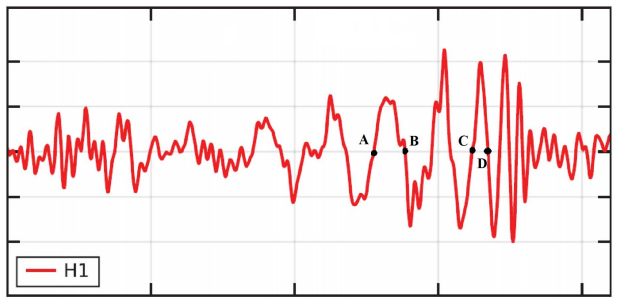
\includegraphics[width=0.7\linewidth]{imagens/grafico OG 1.png}
        \caption{Deformação, ou seja, variação relativa do tamanho de cada braço, no detector LIGO H1. O eixo horizontal representa o tempo, e os pontos A, B, C, D correspondem a \(t = 0,000\), \(0,009\), \(0,034\), \(0,040\) segundos, respectivamente.}
    \end{figure}

    \item A partir da figura, estime \( f_{OG}(t) \) em:

    \[
    t_{AB} = \frac{t_B + t_A}{2} \quad \text{e} \quad t_{CD} = \frac{t_D + t_C}{2}.
    \]
    
    Assumindo que a equação para \(f_{OG}\) é válida até a colisão (o que, estritamente falando, não é verdade) e que os dois objetos possuem massas iguais, estime a massa "chirp", \( M_c \), e a massa total do sistema, em termos de massas solares \( M_\odot \simeq 2 \times 10^{30} \, \text{kg}\).

    \item Estime a separação orbital mínima entre os dois objetos em \( t_{CD} \). 
    Assim, estime um tamanho máximo para cada objeto, \( R_{\text{max}} \). 
    Obtenha \( \frac{R_\odot}{R_{\text{max}}} \) para comparar esse tamanho com o raio do nosso Sol, \( R_\odot \simeq 7 \times 10^5 \, \text{km} \). 
    Estime também sua velocidade orbital linear no mesmo instante, \( v_{\text{col}} \), comparando-a com a velocidade da luz, \( \frac{v_{\text{col}}}{c} \).
\end{alternativas}

\begin{pssolution*}{}{}
    \begin{alternativas}
        \item Da segunda lei de newton, 
        \[-\frac{GM_1M_2}{(r_1+r_2)^3}\mathbf{d} = M_1\mathbf{a_1}\]

        Onde \(\mathbf{d}\) é um vetor que saí da estrela dois e vai até a estrela um. Portanto, \(|\mathbf{d}| = r_1+r_2\). Utilizando o teorema do centro de massa, temos 

        \[r_2 = \frac{M_1r_1}{M_2}\]

        Substituindo e simplificando, 

        \[\mathbf{a_1} = -\frac{GM_2}{r_1^3(1+\frac{M_1}{M_2})^3}\mathbf{d}\]

        Agora trabalhando no vetor \(\mathbf{d}\), note que a sua direção é a mesma direção que \(\mathbf{r_1}\), uma vez que a linha que liga 1 e 2, obrigatóriamente passa pelo CM do sistema. Assim, 

        \[\mathbf{d} = |\mathbf{d}|\hat{\mathbf{r_1}} = (r_1+r_2)\hat{\mathbf{r_1}} = (1+M_1/M_2)\mathbf{r_1}\]

        Substituindo, 

        \[\mathbf{a_1} = -\frac{GM_2}{(1+M_1/M_2)^2}\frac{\mathbf{r_1}}{r_1^3}\]

        Com isso, podemos concluir que 

        \[\boxed{\alpha = \frac{GM_2}{(1+M_1/M_2)^2}, \ \ \ n = 3 \ }\]

        \item A energia do sistema é dada por, 
        \[E = \frac{M_1v_1^2+M_2v_2^2}{2}-\frac{GM_1M_2}{L}\]

        Focando no primeiro termo e utilizando-se de que, \(v_A = r_A\omega\), temos 

        \[M_1v_1^2+M_2v_2^2 = (M_1r_1^2 + M_2r_2^2)\omega^2 \]

        Pelo teorema do centro de massa 

        \[(M_1r_1-M_2r_2)^2=0 \rightarrow M_1r_1^2 +M_2r^2_2 = \frac{M_1M_2}{M_1+M_2}L^2\equiv \mu L^2\]

        Para o segundo termo, basta multiplicar em cima e embaixo por \((M_1+M_2)\). Assim, 

        \[E = \frac{\mu L^2}{2} - \frac{G}{L}\frac{M_1M_2}{M_1+M_2}(M_1+M_2) \equiv \frac{\mu L^2\omega^2}{2} + \frac{GM\mu }{L}\]

        Desse modo, \(\boxed{A = \frac{\mu L^2\omega^2}{2}}\).

        \item Pela terceira lei de kepler, 
        
        \[\omega^2 = \frac{GM}{L^3}\]

        Substituindo, 

        \[E = \frac{GM\mu}{2L} - \frac{GM\mu}{L} = -\frac{GM\mu}{L}\]

        Concluindo assim, que \(\boxed{\beta = -1/2}\).

        \item Seja, \(\theta\) o ângulo que o vetor \(r_1\) faz com o eixo \(x\), desse modo, 
        \[(x_1, \ y_1) = r_1(\cos\theta, \ \sin\theta)\]

        O vetor \(r_2\) deve fazer um ângulo de \(\pi + \theta\). Utilizando que \(\sin(\pi+\theta) = -\sin(\theta)\) e \(\cos(\pi+\theta) = -\cos\theta\), 

        \[(x_2, \ y_2) = -r_2(\cos\theta, \sin\theta)\]

        Definindo por \(t\) o tempo decorrido desde que as estrelas cruzaram o eixo \(x\), tem se \(\theta = \omega t\). Logo, 

        \[\boxed{(x_1, \ y_1) = r_1 (\cos(\omega t), \ \sin(\omega t)) \ \ \ (x_2, \ y_2) = -r_2 (\cos(\omega t), \ \sin(\omega t))}\]

        \item A matrix terá a seguinte cara, 
        
        \[Q = \left(\begin{matrix}
            Q_{11} & Q_{12} & Q_{13} \\
            Q_{21} & Q_{22} & Q_{23} \\
            Q_{31} & Q_{32} & Q_{33} \\
        \end{matrix}\right)\]

        Evocando as fórmulas do enunciado, 
        \[
        Q_{11} = \sum_{A=1}^2 \frac{M_A}{3} \left( 2x_A^2 - y_A^2 \right),
        \]

        \[
        Q_{22} = \sum_{A=1}^2 \frac{M_A}{3} \left( 2y_A^2 - x_A^2 \right),
        \]

        \[
        Q_{33} = -\sum_{A=1}^2 \frac{M_A}{3} \left( x_A^2 + y_A^2 \right),
        \]

        \[
        Q_{12} = Q_{21} = \sum_{A=1}^2 M_A x_A y_A.
        \]

         Para \(Q_{11}\), temos, 

        \[Q_{11} = \frac{M_1}{3}(2x_1^2-y_1^2) + \frac{M_2}{3}(2x_2^2-y_2^2)\]

        Substituindo \(x\) e \(y\), 

        \[Q_{11} = \frac{M_1}{3}r_1^2(2\cos^2(\omega t) - \sin^2(\omega t)) + \frac{M_2r^2_2}{3}(2\cos^2(\omega t) - \sin^2(\omega t))\]

        \[Q_{11} = \frac{1}{3}(2\cos^2(\omega t) - \sin^2(\omega t))(M_1r_1^2 + M_2r_2^2)\]  
        \[Q_{11} = \frac{\mu L^2}{3}(2\cos^2(\omega t) - \sin^2(\omega t))\]

        Para \(Q_{22}\), 

        \[Q_{22} = \frac{M_1r_1^2}{3}(2\sin^2(\omega t) - \cos^2(\omega t)) + \frac{M_2r_2^2}{3}(2\sin^2(\omega t) - \cos^(\omega t))\]

        \[Q_{22} = \frac{\mu L^2}{3}(2\sin^2(\omega t) - \cos^2(\omega t))\]


        Para \(Q_{33}\)

        \[Q_{33} = -\frac{M_1r_1^2}{3}(\cos^2(\omega t) + \sin^2(\omega t))-\frac{M_2r_2^2}{3}(\cos^2(\omega t) + \sin^2(\omega t))\]

        \[Q_{33} = -\frac{\mu L^2}{3}\]

        Por fim, para \(Q_{12} = Q_{21}\), 

        \[Q_{12} = Q_{21} = M_1r_1^2\cos(\omega t) \sin(\omega t) + M_2r_2^2\cos(\omega t)\sin(\omega t)\]

        \[Q_{12} = Q_{21} = \mu L^2 \sin(\omega t)\cos(\omega t) = \frac{\mu L^2}{2}\sin(2\omega t)\]

        Como os de mais termos são \(0\), podemos escolher como \(A\) o valor de\(\mu L^2/2\), assim a nossa matriz \(Q\) toma forma, 

        \[Q = \frac{\mu L^2}{2}\left(\begin{matrix}
            \frac{4}{3}\cos^2(\omega t) - \frac{2}{3}\sin^2(\omega t)  & \sin(2\omega t) & 0 \\
            \sin(2\omega t) & \frac{4}{3}\sin^2(\omega t) - \frac{2}{3}\cos(\omega t) & 0 \\
            0 & 0 & -\frac{2}{3} \\
            \end{matrix}\right)\]

        Para os termos \(a_{11}\) e \(a_{22}\), vamos utilizar identidades trigonométricas, começando com \(a_{11}\), 
        \[\frac{4}{3}\cos^2(\omega t) - \frac{2}{3}\sin^2(\omega t) = \frac{2}{3}(2\cos^2(\omega t) - \sin^2(\omega t))\]

        Usando \(\cos^2(\omega t) = 1-\sin^2(\omega t)\), temos, 

        \[ = \frac{2}{3}\left(2-3\sin^{2}(\omega t)\right)\]

        Usando a forma do arco duplo, temos, 

        \[\cos(2x) = \cos^2x -\sin^2x = 1-2\sin^2x \rightarrow \sin^2x = \frac{1-\cos(2x)}{2}\]

        Fazendo essa substituição, 

        \[=\frac{2}{3}\left(2 - \frac{3}{2} + \frac{3}{2}\cos(2\omega t)\right) = \frac{1}{3}+\cos(2\omega t)\]

        Utilizando o mesmo processo para \(a_22\), encontramos
        \[a_{22} = \frac{1}{3}-\cos(2\omega t)\]

        De modo que nossa matriz pode ser simplificada para, 


        \[\boxed{Q = \left(\begin{matrix}
            \frac{1}{3}+\cos(2\omega t) & \sin(2\omega t) & 0 \\
            \sin(2\omega t) & \frac{1}{3} - \cos(2\omega t) & 0 \\
            0 & 0 & -\frac{2}{3} \\
        \end{matrix}\right)}\]

        \item Analisando a matriz anterior, temos que, 
        \[\boxed{A = \frac{\mu L^2}{2}}\]
        E que
        \[\boxed{b_1 = b_2 = \frac{1}{3}, \ \ b_3 = -\frac{2}{3}, \ \ j_1 = 1, \ \ j_2 = -1, \ \ j_3 = 0, \ \ p_{12}=p_{21} = 2, \ \ k= 2}\]

        \item A fórmula fornecida para a potência foi, 
        
        \[
        \mathcal{P} = \frac{G}{5c^5} \sum_{i=1}^3 \sum_{j=1}^3 \left( \frac{d^3 Q_{ij}}{dt^3} \right) \left( \frac{d^3 Q_{ij}}{dt^3} \right).
        \]

        Para começar, vamos derivar a matri \(Q\) com respeito ao tempo, 

        \[\frac{d^3 Q}{dt^3} = \frac{\mu L^2}{2}\frac{d^3}{dt^3}\left(\begin{matrix}
            \frac{1}{3}+\cos(2\omega t) & \sin(2\omega t) & 0 \\
            \sin(2\omega t) & \frac{1}{3} - \cos(2\omega t) & 0 \\
            0 & 0 & -\frac{2}{3} \\
        \end{matrix}\right)\]

        Para derivar uma matriz, basta derivarmos todos os seus elemtentos, ao fazer isso, chegamos em, 

        \[\frac{d^3Q}{dt^3} = \frac{\mu L^2}{2}\left(\begin{matrix}
            8\omega^3 \sin(2\omega t) & -8\omega ^3\cos(2\omega t) & 0 \\
            -8\omega^3\cos(\omega t) & -8\omega^3\sin(\omega t) & 0 \\
            0 & 0 & 0 \\ 
        \end{matrix}\right)\]

        Deixando o termo em como fora da matriz, 

        \[\frac{d^3Q}{dt^3} = 4\mu\omega^3L^2\left(\begin{matrix}
            \sin(2\omega t) & - \cos(2\omega t) & 0 \\
            -\cos(2\omega t) & - \sin(\omega t) & 0 \\
            0 & 0 & 0 \\
        \end{matrix}\right)\]

        Foi fornecido como dica que o termo 

        \[\sum_{i=1}^3 \sum_{j=1}^3 \left( \frac{d^3 Q_{ij}}{dt^3} \right) \left( \frac{d^3 Q_{ij}}{dt^3} \right)\]

        Corresponde a soma quadradica dos membros da matriz, desse modo 

        \[\sum_{i=1}^3 \sum_{j=1}^3 \left( \frac{d^3 Q_{ij}}{dt^3} \right) \left( \frac{d^3 Q_{ij}}{dt^3} \right) = (4\mu \omega^3 L^2)^2(\sin^2(2\omega t) + 2 \cos^2(\omega t))\]

        Assim, 

        \[\mathcal{P} = \frac{G}{5c^5} \sum_{i=1}^3 \sum_{j=1}^3 \left( \frac{d^3 Q_{ij}}{dt^3} \right) \left( \frac{d^3 Q_{ij}}{dt^3} \right) = \frac{G}{5c^5}(32\mu^2\omega^6 L^4)\]

        Reorganizando, 

        \[\mathcal{P} = \frac{32}{5}\frac{G\mu^2\omega^6L^4}{c^5}\]

        Comparando essa expressão com a fornecida pelo enunciado, temos, 

        \[\boxed{\xi = \frac{32}{5}}\]

        \item \(\mathcal{P}\) representa a potência que está sendo dissipada pelas OG's, assim, 
        \[\mathcal{P} = -\frac{dE}{dt}\]

        Igualando \(E\) a energia da órbita, 

        \[\mathcal{P} = \frac{GM\mu}{2} \frac{d}{dt}\frac{1}{L}\]

        Podemos escrever \(\omega\) em função de \(L\), para isso, basta utilizar a terceira lei de kepler, 


        \[\omega^2 = \frac{GM}{L^3} \rightarrow \frac{1}{L }= (GM)^{-1/3}\omega^{2/3}\]

        Substituindo, 

        \[\mathcal{P} = \frac{(GM)^{2/3}\mu}{2}\frac{d}{dt}\omega^{2/3} = \frac{(GM)^{2/3}\mu}{2}\frac{d}{d\omega}\omega^{2/3}\frac{d\omega}{dt}\]

        \[= \frac{(GM)^{2/3}\mu}{3\omega^{1/3}}\frac{d\omega}{dt}\]

        Igualando a expressão obtida no item anterior, 

        \[\frac{\xi G\mu^2\omega^6L^4}{c^5} = \frac{(GM)^{2/3}\mu}{3\omega^{1/3}}\frac{d\omega}{dt}\]

        Resolvendo para \(d\omega/dt\), 
        
        \[\frac{d\omega }{dt} = (3\xi)\frac{G\mu \omega^{19/3}L^4}{(GM)^{2/3}c^5}\]

        Substituindo \(L = \left(\frac{GM}{\omega^2}\right)^{1/3}\), temos, 

        \[\frac{d\omega}{dt} = (3\xi)\frac{G\mu \omega^{19/3}}{(GM)^{2/3}c^5}\left(\frac{GM}{\omega^2}\right)^{4/3}\]

        Elevando ao cubo, 

        \[\left(\frac{d\omega}{dt}\right)^{3} = (3\xi)^3\frac{G^3\mu^3\omega^{19}}{G^2M^2c^{15}}\frac{G^4M^4}{\omega^8}\]

        Simplificando, 

        \[\boxed{\left(\frac{d\omega}{dt}\right)^3 = (3\xi)^3\frac{\omega^{11}}{c^{{15}}}(G^5\mu^3M^2)}\]

        Analisabdo a expressão do enunciado, temos, 

        \[\boxed{M_c = (\mu^3 M^2)^{1/5}}\]

        \item Utilizando o fato fornecido pelo enunciado, 
        
        \[\frac{d F(t)}{dt} = \chi F(t)^a \rightarrow F(t)^{1-a} = \chi (1-a)(t_0-t)\]

        Podemos encontrar uma expressão para \(\omega(t)\).

        \[\frac{d\omega}{dt} = \frac{3\xi (GM_c)^{3/5}}{c^5}\omega^{11/3} \rightarrow \omega^{1-11/3} = \frac{3\xi (GM_c)^{3/5}}{c^5}(1-11/3)(t_0-t)\]

        Simplificando, 

        \[\omega ^{-8/3} = -\frac{3\xi (GM_c)^{3/5}}{c^5}\frac{8}{3}(t_0-t)\]

        \[\omega^{-8/3} = \frac{8\xi (GM_c)^{3/5}(t-t_0)}{c^5}\]

        Para encontrar uma expressão para \(f_{OG}\), temos que utilizar que, 

        \[f_{OG} = 2f_{orbt} = \frac{\omega}{\pi}\rightarrow \omega = \pi f_{OG}\]

        Fazendo tal substituição, chegamos em, 


        \[f_{OG}^{-8/3} = \frac{8\pi^{8/3}(GM_c)^{3/5}(t-t_0)}{c^5}\]

        Comparando com a forma do enunciado, podemos obter, 

        \[\boxed{p = 1}\]

        \item  A partir da figura, consideramos os dois $\Delta t$ como meias-períodos. Assim, a frequência de onda gravitacional cíclica é $f_{OG} = 1/(2 \Delta t)$. Então, os quatro pontos fornecidos nos permitem calcular a frequência no tempo médio dos dois intervalos como:

        \[
        \begin{array}{|c|c|}
        \hline
        t \, (\text{s}) & f_{OG} \, (\text{Hz}) \\
        \hline
        t_{AB} = 0.0045 & f_{OG}(t_{AB}) = (2 \times 0.009)^{-1} \\
        t_{CD} = 0.037 & f_{OG}(t_{CD}) = (2 \times 0.006)^{-1} \\
        \hline
        \end{array}
        \]
        
        Agora, temos dois pares de valores $(f_{OG}, t)$ para duas incógnitas $(t_0, M_c)$. Em termos de $t_{AB}$ e $t_{CD}$ e dividindo as duas equações, obtemos:
        
        \[
        t_0 = \frac{A t_{CD} - t_{AB}}{A - 1}, \quad A = \left( \frac{f_{OG}(t_{AB})}{f_{OG}(t_{CD})} \right)^{-8/3}.
        \]
        
        Substituindo os valores numéricos, $A \simeq 2.95$ e $t_0 \simeq 0.054 \, \text{s}$. Agora podemos usar a equação de \(f_{OG}\) para qualquer um dos valores $t_{AB}$ ou $t_{CD}$ e determinar $M_c$. Obtém-se a massa de chirp:
        
        \[
        M_c \simeq 6 \times 10^{31} \, \text{kg} \simeq 30 \, M_\odot\]
        
        Assim, a massa total $M$ é:
        
        \[
        M = 4^{3/5} M_c \simeq 69 \, M_\odot
        \]
        
        Este resultado é, na verdade, notavelmente próximo das melhores estimativas usando a teoria completa da Relatividade Geral! [Mesmo que os objetos reais não tenham massas exatamente iguais e a teoria que acabamos de usar não seja válida muito próximo da colisão.]
    
        \item Usando a lei de Kepler estabelece que $L = (GM / \Omega^2)^{1/3}$. O segundo par de pontos destacados no gráfico corresponde ao ciclo anterior à fusão. Assim, utilizando que \(f_{OG} = \omega/\pi\), 

        \[
        \omega_{t_{CD}} \sim 2.6 \times 10^2 \, \text{rad/s}.
        \]
        
        Em seguida, usando a massa total obtida anteriormente:
        
        \[
        L \sim 5 \times 10^2 \, \text{km}
        \]
        
        Assim, esses objetos possuem um raio máximo de $R_{\text{max}} \sim 250 \, \text{km}$. Portanto, eles têm mais de 30 vezes mais massa e:
        
        \[
        \frac{R_\odot}{R_{\text{max}}} \sim 3 \times 10^3,
        \]
        
        eles são 3000 vezes menores que o Sol!
        
        A velocidade linear é:
        
        \[
        v_{\text{col}} = \frac{L}{2} \omega \simeq 7 \times 10^4 \, \text{km/s}. 
        \]
        
        Eles estão se movendo a mais de 20\% da velocidade da luz!
        
        \[
        \boxed{
        \begin{aligned}
        \quad & L_{\text{col}} \sim 5 \times 10^2 \, \text{km}, \\
        & \frac{R_\odot}{R_{\text{max}}} \sim 3 \times 10^3, \\
        & \frac{v_{\text{col}}}{c} \sim 0.2.
        \end{aligned}
        }
        \]
    \end{alternativas}
    
\end{pssolution*}
\end{pproblem}

\pts{3}
\begin{pproblem}(Barra 2024) Durante sua estadia no Hotel Fazenda Ribeirão, Hugo observava a estrela Plo I com seu telescópio. Comparando o seu espectro com o de outras estrelas, ele descobre que Plo I é uma estrela de nêutrons e estima sua massa como sendo \( M_1 = 2M_{\odot} \). Ele também observa que Plo I possui variações senoidais em sua velocidade radial ao longo do tempo e conclui que Plo I deve fazer parte de um sistema binário com outro corpo celeste, Plo II. Observando a curva de velocidade de Plo I, Hugo também determina que Plo I possui uma órbita circular de período \( P \) e velocidade radial máxima \( K \). Porém, ele não sabe qual é a massa \( M_2 \) de Plo II e nem qual é a inclinação \( i \) do plano orbital do binário em relação ao plano do céu, representada na figura a seguir.

    \begin{figure}[H]
        \centering
        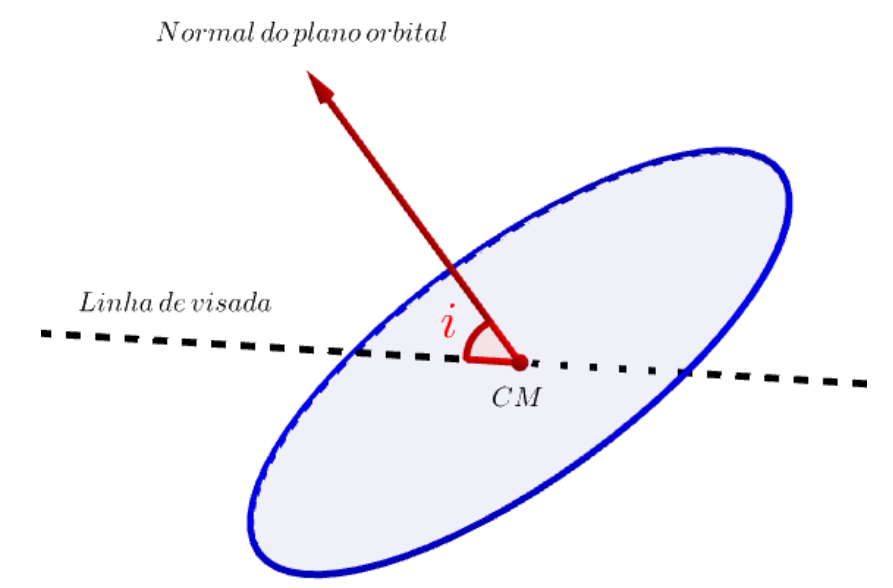
\includegraphics[width=0.8\linewidth]{imagens/figurabarra.png}
        \caption{Representação da órbita}
    \end{figure}

    \begin{alternativas}
        \item A partir da 3ª lei de Kepler e da 2ª lei de Newton, encontre uma expressão para a \textbf{função de massa} do sistema binário formado por Plo I e Plo II em termos de \( P \), \( K \) e constantes universais. Você pode utilizar que a função de massa é dada por:
        \[
            f = \frac{M_2^3 \sin^3 i}{(M_1 + M_2)^2}
        \]
    
        \item Utilizando suas medidas, Hugo calcula que a função de massa do binário é \( f = 46,2M_{\odot} \). Desejamos encontrar o valor mínimo \( M_{2,\text{min}} \) para a massa de Plo II, sabendo que ele corresponde ao caso em que \( i = 90^\circ \). Suponha \( M_{2,\text{min}} > M_1 \). A partir disso, determine \( M_{2,\text{min}} \). Seu resultado é condizente com a hipótese? Responda SIM ou NÃO, justificando com cálculos.
        
        \item Com base em sua resposta do item anterior, conclua: é mais provável que Plo II seja um exoplaneta, uma anã branca, uma estrela de nêutrons ou um buraco negro?
    \end{alternativas}
    \begin{pssolution*}{}{}
        \begin{alternativas}
            \item Primeiramente, note que \(v_{r, aparente} = |\mathbf{\omega}\times\mathbf{r}| = \omega r \sin i = v_r \sin i\), logo \(K = v_r\sin i = \frac{2\pi a_1}{T}\sin i\). Defindino \(a=a_1+a_2\) e \(M = M_1+M_2\) onde \(a_i\) e \(M_i\) representam a distância entre a estrela \(i\) e o CM e a massa da estrela \(i\), temos a terceira lei de kepler como, 
            \[\frac{a^3}{T^2} = \frac{GM}{4\pi^2}\]

            \[a^3 = \frac{GM}{4\pi^2}T^2 \rightarrow T = 2\pi \sqrt{\frac{a^3}{GM}}\]

            Substituindo $T = \frac{2\pi a_1}{v_1}$

            $$(a_1+a_2)^3= \frac{G(M_1+M_2)a_1^2}{v_1^2}$$

            $$(1+a_2/a_1)^2 = \frac{G(M_1+M_2)}{(a_1+a_2)v_1^2}$$

            Também, usando o teorema do centro de massa, 

            $$\frac{a_1}{a_2} = \frac{M_2}{M_1}$$

            Trabalhando na função de massa, 

            $$\frac{1}{f} = \frac{(1+M_1/M_2)^2}{M_2\sin^3 i} = \frac{(1+a_2/a_1)^2}{M_2\sin^3i}$$

            Substituindo $(1+a_2/a_1)$

            $$\frac{1}{f} = \frac{G(M_1+M_2)}{(a_1+a_2)M_2v_1^2\sin^3i} = \frac{G(1+M_1/M_2)}{(a_1+a_2)v_1^2\sin^3i} = \frac{G(1+a_2/a_1)}{(a_1+a_2)v_1^2\sin^3i}$$

            Substituindo $(1+a_2/a_1)$ novamente, 

            $$\frac{1}{f} = \frac{G}{v_1^3\sin^3i}\sqrt{\frac{G(M_1+M_2)}{(a_1+a_2)^3}}$$

            Mas olhe a similaridade do termo dentro da raiz com a terceira lei de kepler! Assim, 

            $$\frac{1}{f} = \frac{2\pi G }{T v_1^3\sin^2i}$$

            Finalmente, substituindo K e reajeitando, 

            $$\boxed{f = \frac{TK^3}{2\pi G}}$$

            \item Suponto $i = 90^\circ$, temos 
            
            $$f = \frac{M_2^3}{(M_1+M_2)^2}$$

            Usando unidades de massas solares e $M_1 = 2M_\odot$, temos, 

            $$46,2 = \frac{M_2^3}{(2+M_2)^2}$$

            $$M_2 = \left(46,2 (2+M_2)^2\right)^{1/3}$$

            Usando iteração podemos encontrar $\boxed{M_2 = 49,7 M_\odot }$

            \item Como a massade \(M_2\) é muito grande, é mais provavel de que o mesmo se trate de um buraco negro
        \end{alternativas}
    \end{pssolution*}
\end{pproblem}

\pts{3}
\begin{pproblem} Juventino está localizado na sua base (não tão) secreta no Polo Norte terrestere. Após uma chama de emergencia de deduardo letodo, o mesmo precisa mandar um missél para o equador, afim de explodir a base de seu arqui inimigo: Raposo. 
    \begin{alternativas}
        \item Junvetino não está na sua melhor forma, e com toda a sua força, ele só consegue arremessar o foguete na primeira velocidade cósmica (a velocidade orbital para corpos próximos da superfície terrestre). Nessas condições, qual é o semi eixo da órbita do foguete lançado por Juventino?
        \item Qual a maior altura que o foguete chega?
        \item Qual o intervalo de tempo entre o Juventino lançar o foguete e a base de Raposo ser explodida?
    \end{alternativas}
    
\end{pproblem}

\pts{5}
\begin{pproblem}
    Nesse problema, nosso objetivo será calcular o período de precessão da Terra. Para isso, vamos considerar a Terra como um elipsoide, com raio polar $R_p$, raio equatiorial $R_e$, com período de rotação em torno do eixo polar $T = 23^h56^m4^s$ e massa $M_\oplus$ uniformemente distribuida. Para o nosso modelo, considere que apenas o Sol e a Lua exercem forças gravitacionais relevantes para o problema.
    \begin{alternativas}
        \item Considerando que $R_p = R_\oplus\approx 6371 \text{ km}$, qual o valor numérico de $R_e$?
        
        \item O momento de inercía de um corpo, pode ser calculado por $I = \int r^2 dm$. Sabendo disso, calcule o momento de inercia no eixo x e no eixo z de um elipsoide dado pela equação 
        $$\frac{x^2}{R_e^2} + \frac{y^2}{R_e^2} + \frac{z^2}{R_p^2}= 1$$
        Com os momentos de inercia calculados, para a Terra, vamos definir o eixo $x$ como o eixo que contem o equador e o eixo $y$ como aquele que contem os polos. Calcule a quantidade, 
        $$\frac{I_p}{(I_p-I_e)}$$

        Onde $I_p$ é o momento de inercia polar (no eixo y) e $I_e$ o momento de inceria equatorial (no eixo y). Assuma que a terra seja homogênea. Devido a assompção de uma Terra homogênea, a sua quantia será 93\% do que a quantidade real. 
        

        \item Encontre uma expressão para o torque exercicios pelo sistema Sol-Lua na Terra. (Dica, devido a simetria, muitos termos dentro de integrais irão zerar e o torque final terá componente em apenas uma direção no sistema de coordenadas definidos anteriormente)
        \item Por fim, utilizando a equação, 
        $$\vec{\tau} = \Omega \times \mathbf{L} $$
        Onde $\mathbf{L}$ é o momento angular e $\Omega$ é a frequencia de precessão, encontre o período de precessão da Terra.
    \end{alternativas}

    \begin{pssolution*}{}{}
        \begin{alternativas}
            \item Como a Terra está em equilíbrio hidrostático, 
            
            \[\frac{GM_\oplus}{r_p} = \frac{GM_\oplus}{r_e}+\frac{1}{2}\omega^2 r_e^2\]
        
            Resolvendo para \(r_e\), 

            \[r_e = \frac{T}{2\pi}\sqrt{2GM_\oplus\left(\frac{1}{r_p}-\frac{1}{r_e}\right)}\]

            Iterando, podemos obter, 

            \[r_e \approx 6382 \text{ km}\]

            \item Dada a definição do elipsoide, \(x\) e \(y\) estão no plano equatorial e \(z\) passa pelo centro da Terra e pelo polo norte celeste. Calculando os momentos de inércia, 
            
            \[I_{zz} = \int(y^2+z^2)dm = \rho \iiint (x^2+y^2)dxdydz\]

            Usando a transformação, 

            \[x = R_e u \, \ y = R_e v \, \ z = R_p w\]

            De modo que \(u^2+v^2+w^2=1\), temos, 

            \[I_{zz} = \rho\iiint (R_e^2u^2+R_e^2v^2) R_e^2R_pdudvdw = \rho R_e^4R_p \iiint (u^2+v^2)dudvdw\]

            Como \(u^2+v^2+w^2=1\) descreve uma esfera unitária, temos simetria, o que garante, 

            \[\iiint u^2d\Omega = \iint v^2d\Omega = \iint w^2d\Omega = \frac{1}{3}\iiint(u^2+v^2+w^2)d\Omega\]

            Podemos simplificar, 

            \[\frac{1}{3}\iiint(u^2+v^2+w^2)d\Omega = \frac{1}{3}\int_0^{2\pi}\int_{0}^{\pi}\int_0^1 r^4\sin\theta drd\theta d\phi = \frac{4\pi}{15}\]

            Resolvendo para \(I_{zz}\), 

            \[I_{zz} = \rho R_e^4 R_p \left(\frac{4\pi}{15}+\frac{4\pi}{15}\right)\]

            Substituindo \(\rho = 3M_\oplus/4\pi R_e^2R_p\), obtemos, 

            \[I_{zz} = \frac{2}{5}M_\oplus R_e^2\]

            Fazendo a mesma coisa para 

            \[I_{xx} = \rho R_e^2R_p\iiint ((R_ev)^2+(R_pw)^2)dudvdw\]

            Vamos obter 

            \[I_{xx} = \frac{1}{5}M_\oplus(R_e^2+R_p^2)\]

            Note também que \(I_{zz} \equiv I_p\) e \(I_{xx}\equiv I_e\). Desse modo, 

            \[\boxed{\frac{I_e}{I_p-I_e} \approx 580}\]

            Como o nosso valor é \(93\%\) maior do que esperado, temos que na realidade essa quantida deve equivaler há \(\approx 300\). Vamos chamar essa quandidade de \(f\) e seguir com ela daqui pra frente.

            \item Como o torque é tal que
            
            \[\tau \propto \frac{M}{r^3}\]

            Temos 

            \[\frac{\tau_{lua}}{\tau_\odot} = \frac{M_{lua}}{M_\odot}\frac{d_\odot}{d_{lua}}\approx 2,17\]

            Agora, para encontrar o torque do Sol, vamos primeiro calcular a força que ele exerce em um diferencial de massa \(dm\) na Terra. Vamos definir \(\mathbf R\) como o vetor posição do Sol e \(\mathbf r\) o vetor posição do diferencial de massa.

            \[d\mathbf F = -\frac{GM_\odot}{|\mathbf R - \mathbf r|^3}(\mathbf R - \mathbf r)dm\]

            Com relação ao centro da Terra, o torque é 

            \[d\vec\tau = \mathbf r \times d\mathbf F = \frac{GM_\odot}{|\mathbf R - \mathbf r|^3}(\mathbf R \times \mathbf r)dm\]

            Usando que \(R>>r\) e a aproximação \((1+x)^n\approx 1+nx\) obtemos, 

            \[d\vec\tau \approx \frac{GM_\oplus}{R^3}\left(1+3\frac{\mathbf R \cdot \mathbf r}{R^2}\right)(\mathbf R \times \mathbf r )dm\]

            Expandindo o produto vetorial, 

            \[\mathbf R \times \mathbf r = (R_yr_z - R_z r_y )\mathbf{\hat x} + (R_zr_x - R_xr_z)\mathbf {\hat y} + (R_xr_y - R_yr_x) \mathbf{\hat z}\]

            Dessa maneira, 

            \[\tau_x = \frac{GM_\oplus}{R^3}\int \left(1+3\frac{R_xr_x+R_yr_y+R_zr_z}{R^2}\right)(R_yr_z-R_zr_y)dm\]

            Porém quando resolvemos a integral, podemos perceber que todos os termos na forma \(\int r_i dm \) e \(\int r_ir_jdm\) são nulos, devidos a simetria. Por tanto a nossa integral se reduz para 

            \[\tau_x = \frac{3GM_\oplus}{R^5}R_yR_z\left(\int r_y^2dm + \int r_z^2dm\right)\]

            As integrais restantes são os momentos de inercia em \(y\) e \(z\). Similarmente para \(\tau_y\) e \(\tau_z\) obtemos, 

            \[\tau_x = \frac{3GM_\oplus}{R^5}R_yR_z (I_{yy}-I{zz})\]
            \[\tau_y = \frac{3GM_\oplus}{R^5}R_zR_x (I_{zz}-I{xx})\]
            \[\tau_z = \frac{3GM_\oplus}{R^5}R_xR_y (I_{xx}-I{yy})\]

            Podemos descrever \(R_i\) usando o sistema de coordenadas elípticas.

            \[R_x = R\sin\lambda \cos\epsilon\]
            \[R_y = R\cos\lambda\]
            \[R_z = R\sin\lambda\sin\epsilon\]

            Onde \(\lambda\) é a longitude ecliptica do Sol. Assim, 

            \[\tau_x = \frac{3GM_\oplus}{R^3}\sin\lambda\cos\lambda\sin\epsilon (I_{yy}-I_{zz})\]
            \[\tau_y = \frac{3GM_\oplus}{R^3} \sin^2\lambda\sin\epsilon\cos\epsilon(I_{zz}-I_{xx})\]
            \[\tau_z = \frac{3GM_\oplus}{R^3} \sin\lambda\cos\lambda\cos\epsilon(I_{xx}-I_{yy})\]

            Para o efeito de precessão, o importante é o valor médio do torque, porém note que \[\langle\sin\lambda\cos\lambda\rangle = 0\]. Assim, o único toruqe que se mantém é o do eixo \(y\).

            \[\vec\tau  = \langle\tau_y\rangle\mathbf{\hat{y}} = \frac{3GM_\oplus}{2R^3}\sin\epsilon\cos\epsilon (I_{zz}-I_{xx})\mathbf{\hat{y}}\]

            Essa é apenas a contribuição do Sol. Adicionando a da Lua temos, 

            \[\boxed{\vec\tau_{total} = \frac{4,75GM_\oplus}{R^3}\sin\epsilon\cos\epsilon (I_{p}-I_{e})\mathbf{\hat{y}}}\]

            \item Utilizando a relação dada, 
            
            \[\vec\tau_{total} = \vec\Omega \times \vec L = \Omega L_\perp\]

            O valor de \(L_\perp\) é \(I_p\omega\sin\epsilon\). Assim, 

            \[\frac{4,75GM_\oplus}{R^3}\sin\epsilon\cos\epsilon (I_{p}-I_{e}) = \frac{2\pi}{T}I_p\omega\sin\epsilon\]

            Resolvendo para \(T\), 

            \[\boxed{T = \frac{2\pi}{4,75}\frac{R^3\omega}{GM_\oplus\cos\epsilon}\frac{I_p}{I_p-I_e}\approx 25300\text{ anos}}\]

            O que é uma estimativa com apenas \(2\%\) de erro :)
        
        \end{alternativas}
    \end{pssolution*}
\end{pproblem}
    

\end{document}